\documentclass[english,12pt,a4paper]{book}
\usepackage[T1]{fontenc} % In case we want special characters
\usepackage[utf8]{inputenc} % We are all writing in UTF-8

\usepackage[numbers]{natbib} % We need to tweak our referencing a bit.
\usepackage{appendix} % Fixes formatting of appendices
\usepackage[printonlyused]{acronym} % Package to handle the acronym list
\usepackage{graphicx} % We *may* use images
\graphicspath{{images/}} % and it is clean to put them in a separate dir
\usepackage{hyperref} % Internal and external links is nice
\hypersetup{pdfborder=0 0 0} % ..especially without red borders

% Packages and settings for code listings
\usepackage{listings}
\usepackage{caption}
\usepackage{upquote}
\usepackage{xcolor}
\DeclareCaptionFont{white}{\color{white}}
\DeclareCaptionFormat{listing}{\colorbox{gray}{\parbox{\textwidth}{#1#2#3}}}
\captionsetup[lstlisting]{format=listing,labelfont=white,textfont=white}
\lstset{
language=Python,
keywordstyle=\bfseries\ttfamily\color[rgb]{0,0,1},
identifierstyle=\ttfamily,
commentstyle=\color[rgb]{0.133,0.545,0.133},
stringstyle=\ttfamily\color[rgb]{0.627,0.126,0.941},
showstringspaces=false,
basicstyle=\small,
numberstyle=\footnotesize,
numbers=left,
stepnumber=1,
numbersep=10pt,
tabsize=2,
breaklines=true,
prebreak = \raisebox{0ex}[0ex][0ex]{\ensuremath{\hookleftarrow}},
breakatwhitespace=false,
aboveskip={1.5\baselineskip},
columns=fixed,
upquote=true,
extendedchars=true,
frame=bottomline,
inputencoding=utf8
}

% Set equal margins on book style
% \usepackage{layout} % Use \layout to print out the margins (debug)
\usepackage{geometry}
\geometry{bindingoffset=1cm}

% Restyle chapter headers
\usepackage{fix-cm}
\makeatletter
\renewcommand{\@makechapterhead}[1]{%
  \vspace*{50\p@}%
  {\parindent \z@ \raggedright \normalfont
    \vspace{15pt}%
    \ifnum \c@secnumdepth >\m@ne
        %\hfill\huge\scshape \@chapapp\space
        \hfill\fontsize{60}{90}\selectfont \thechapter % Chapter number
        \par\nobreak
        \vskip 20\p@
    \fi
    \interlinepenalty\@M
    \hfill \Huge \scshape #1\par % Chapter title
    \vspace{5pt}
    \hrule
    \nobreak
    \vskip 40\p@
  }}
\makeatother

\author{Eirik Haver \and Pål Ruud}
\title{Project assignment - Tahoe-LAFS with SHA-3 candidates}
\date{\today}

\begin{document}

% Latex-versjon av ITEM rapportmal.
% Lagd av <lasse.karstensen@gmail.com>, desember 2009.
% Lisens: public domain. 
%
\begin{titlepage}
\begin{center}
\textsc{NORWEGIAN UNIVERSITY OF SCIENCE AND TECHNOLOGY\\
FACULTY OF  INFORMATION TECHNOLOGY, MATHEMATICS AND ELECTRICAL ENGINEERING} \\
\vspace{0.5cm} 
% crop-et fra http://www.ntnu.no/infoavdelingen/selvhjelp/logoer/ntnu/NTNU_engelsk_RGB.png

\includegraphics[scale=0.5]{NTNU-logo} \\

\vspace{1.0cm}
{\Huge{PROJECT ASSIGNMENT}}
\vspace{1.0cm}

\begin{tabular}{ p{4cm} p{11cm}}

Students' name:	& Eirik Haver and Pål Ruud \\
Course: & TTM13 \\
Title: & Experimenting with SHA-3 candidates in Tahoe-LAFS \\
%\vspace{1cm}
Description: & \\
\end{tabular}
{\small{\begin{tabular}{p{15cm}}
\vspace{0.2cm}

Tahoe-LAFS is a Free Software/Open Source decentralized data store. It
distributes your filesystem across multiple servers, and even if some of the
servers fail or are taken over by an attacker, the entire filesystem continues
to work correctly and to preserve your privacy and security.
\\\\
One of the basic security components used in Tahoe-LAFS is the cryptographic
hash function SHA-256.
\\\\
In the light of the worldwide SHA-3 hash competition, this task is about
making a reproducible, automated benchmark which shows how the performance of
Tahoe-LAFS is affected by the performance of the different SHA-3 candidate hash
functions. Before any testing can be done, Python bindings to the C
implementations of the SHA-3 candidates have to be made, since Tahoe-LAFS is
written in the Python programming language.
\\\\
\end{tabular}  }}

\begin{tabular}{ p{4cm} p{11cm}}
Deadline: & 2010-12-xx \\
Submission date: & 2010-12-xx \\
Department: & Department of Telematics \\
Supervisor: & Danilo Gligoroski \\\\
\end{tabular}
\vspace{0.5cm}

Trondheim, \today 

\vspace{0.4cm}
\line(1,0){150} \\
Danilo Gligoroski, NTNU/ITEM. 

\end{center}
\end{titlepage}


\pagestyle{empty}

\chapter*{Abstract}
\addcontentsline{toc}{chapter}{Abstract}
\pagestyle{plain}
\pagenumbering{Roman}
\setcounter{page}{1}

%  Writers should follow a checklist consisting of:
% Motivation: Why do we care about the problem and results?
% Problem Statement: What problem are we trying to solve? Scope/limits.
% Approach: How did we go about solving or making progress on the problem?
% Results: What is the answer? Numbers, not vague 'very', 'small' etc.
% Conclusions: What are the implications of your answer? Further work.
%
%  Each section is typically a single sentence, although there is room for
%  creativity.

Most of the cloud applications today are highly dependant on the use of
cryptographic hash functions. The distributed file system Tahoe-LAFS is no
exception, and uses hashing algorithms extensively for verification of the
integrity of its files.

In light of the ongoing NIST competition for selecting the new, standard
cryptographic hash function named SHA-3, we tried out the 14 second
round candidates in the Tahoe-LAFS file system using automated tests to measure
the performance differences. Only the immutable file support was tested.

Since the Tahoe-LAFS is programmed in Python, we had to make bindings to the
SHA-3 implementations written in C, before making the necessary changes to the
Tahoe-LAFS code. Several tasks where automated using scripts, to avoid doing
manual work of distributing changes to the test grid.

In general, four of the candidates perform better than the currently used
SHA-256 -- BLAKE, BlueMidnightWish, Shabal and Simd.
By utilizing the performance improvements given by SHA-3, Tahoe-LAFS could
save $5\%$ on upload operations by changing hashing function to the best
performing candidate.

The benchmarking tool SUPERCOP measures performance and drives the development
forwards for the SHA-3 candidates, but we argue that since the SUPERCOP API does
not conform with the NIST SHA-3 API, vital functionality are left out, making
integration and testing with existing software hard.

\chapter*{Preface}
\addcontentsline{toc}{chapter}{Preface}

The work behind this project report was carried out during the autumn semester
in 2010 at the Norwegian University of Science and Technology (NTNU), Department
of Telematics (ITEM).
\vspace{13pt}

We would like to thank our fellow classmates for interesting discussions and a
lot of fun as the time and semesters fly by.
\vspace{13pt}

Secondly, we would like to state our appreciation to our supervisor, Danilo
Gligoroski, and his coworker on Blue Midnight Wish, Rune E. Jensen, for
providing useful feedback and interesting stories from the cryptographic
community.
\vspace{13pt}

Lastly, the Open Source community behind Tahoe-LAFS deserves credit for the
immense amount of hours they put on an awesome project, and Thomas Pornin for
providing a working copy of his library of implementations, which saved us a lot
of work.
\vspace{13pt}

Best regards,

\begin{center}
Eirik Haver and Pål Ruud
\vspace{13pt}

December 16, 2010
\end{center}

\tableofcontents

\cleardoublepage
\phantomsection
\addcontentsline{toc}{chapter}{\listfigurename}
\listoffigures

\cleardoublepage
\phantomsection
\addcontentsline{toc}{chapter}{\listtablename}
\listoftables

\cleardoublepage
\phantomsection
\addcontentsline{toc}{chapter}{\lstlistlistingname}
\lstlistoflistings
\cleardoublepage

\chapter*{Acronyms}
\addcontentsline{toc}{chapter}{Acronyms}

\begin{acronym}
\acro{AES}{Advanced Encryption Standard}
\acro{API}{Application programming interface}
\acro{BMW}{Blue Midnight Wish}
\acro{CEB}{Capability Extension Block}
\acro{CPU}{Central Processing Unit}
\acro{Distutils}{Python Distribution Utilities}
\acro{FEC}{Forward Error Correction}
\acro{GCC}{GNU Compiler Collection}
\acro{KAT}{Known Answer Test}
\acro{LAFS}{Least-Authority Filesystem}
\acro{NIST}{National Institute of Standards and Technology}
\acro{RAM}{Random Access Memory}
\acro{RAID}{Redundant Array of Independent Disks}
\acro{SHA}{Secure Hash Algorithm}
\acro{SSE2}{Streaming SIMD Extensions 2}
\acro{SSSE3}{Supplemental Streaming SIMD Extensions 3}
\acro{SUPERCOP}{System for Unified Performance Evaluation Related to
Cryptographic Operations and Primitives}
\acro{SVN}{Subversion}
\acro{UEB}{URI Extension Block}
\acro{URI}{Uniform Resource Identifier}
\end{acronym}

%**************************************%
\chapter{Introduction}
%**************************************%
\pagenumbering{arabic}
\setcounter{page}{1}

The process of selecting what is to become the new standard for a secure hashing
algorithm is carried out by the {NIST}, and is at its final stages at the time
of writing. Fourteen candidates came through to the second round
\cite{s_nistround2}.

The Tahoe-\ac{LAFS} is a distributed, secure file system perfectly suited to
build file sharing services over the Internet. Currently it uses the
\ac{SHA}-256 algorithm to verify the integrity of files and shares, in addition
to creating keys, \ac{URI}s and more \cite{t_tahoe}.

In this project assignment, we integrate the fourteen \ac{SHA}-3 candidates in
the Tahoe-\ac{LAFS} and measure the performance impact. To be able to do this,
we create Python bindings for the best suited C implementations of the SHA-3
candidates, and alter the hash function calls in the source code of Tahoe.

\section{Method}

All work associated with the project has been carried out by the two authors in
cooperation. Code are written using the VIM editor on Ubuntu Linux
driven machines, and version-controlled using the distributed revision control
system Git. All material produced, including this paper, are publicly available
on GitHub\footnote{\url{http://github.com/ruudud/Tahoe-LAFS-with-SHA-3}}.

The \ac{SHA}-3 candidates are tested on the Tahoe-\ac{LAFS} using uploading and
downloading of files on four desktop computers. Various file sizes are used to
simulate different use cases, and to broaden the perspective as to how the
different candidates perform and behaves when implemented in a secure,
distributed file system.

\section{Outline}

The work is presented as per the following chapters:

\paragraph{Chapter 2} provides background knowledge of the technologies and
software used.

\paragraph{Chapter 3} outlines the procedure taken to be able to do the
measurements.

\paragraph{Chapter 4} presents the actual results, in the form of graphs and
tables, in addition to some easily seen conclusions.

\paragraph{Chapter 5} discusses the results and our technical procedure to the
problem presented in this assignment.

\paragraph{Chapter 6} concludes the results and the work done, and proposes
future work.


%**************************************%
\chapter{Background technologies}
%**************************************%

\section{Cryptographic Hash Functions}

A cryptographic hash function is a deterministic mathematical procedure which
takes an arbitrary block of data and outputs a fixed-size bit string. The output
is referred to as the hash value, message digest or simply digest.
Another property of a cryptographic hash function is that the smallest change in
the input data (e.g. one bit) should completely change the output of the hash
function. In other words it should be infeasible to find the reverse of a
cryptographic hash function \cite[p. 335]{stallings}. It should also be infeasible to
find two blocks of data which produce the same hash value (a \emph{collision}).

\subsection{NIST SHA-3 Competition}
The \ac{SHA} version 3 is a coming standard set to supersede the current
standards that the \ac{SHA}-1 and the \ac{SHA}-2 family has become. The hash
function that will be known as \ac{SHA}-3 will be decided by the \ac{NIST} and
chosen between the submitted contestants to the \ac{NIST} hash competition.
At the time of writing, the current status of the competition is officially
called Round 2, with 14 of 64 candidates having ``survived'' Round 1
\cite{s_fedreg}.

\subsubsection{\ac{NIST} evaluation criteria for \ac{SHA}-3}

\label{sec:lengthextension}
\paragraph{Security.} The most important criterion for the SHA-3
candidates\cite{s_nistround2} is security. \citet{s_fedreg} lays out the full
description of security criteria, however the most noteworthy criterion
in regards to Tahoe-\ac{LAFS} is that \ac{SHA}-3 candidates are required to have
resistance against length-extension attacks. Both \ac{SHA}-1 and the \ac{SHA}-2
family are vulnerable to this kind of attack, and thus requires
Tahoe to run the algorithm twice, as described by \citet{schneier}.

\paragraph{Cost and Performance.} Cost and Performance are considered to be the
2nd most important criterion. The absolute minimum for performance is that the
SHA-3 candidate should be faster than the functions in the \ac{SHA}-2 family.
Cost is a measure of how much memory an implementation requires in software,
both the implementation itself and the use of \ac{RAM} during runtime. Another
measure of cost is how many logic gates it takes to implement the function in
hardware.

\paragraph{Algorithm and implementation characteristics.} By this 3rd criterion,
\ac{NIST} emphasizes that algorithms with greater flexibility will be given
preference over other algorithms \cite{s_nistround2}. By flexible, they imply
the possibility of the function to run efficiently on a variety of platforms,
and to use parallelism and instruction set extensions. Another key point of a
flexible hash function is that it should have a simple and elegant design to
encourage understanding, analysis and design confidence.

\subsubsection{\ac{NIST} \ac{SHA}-3 \ac{API}} \ac{NIST} required that every
submission should conform to a specified \ac{API}\cite{s_fedreg}. The \ac{API}
specification \cite{s_nistapi} states in shortness that it requires every
candidate to implement four functions:

\begin{verbatim}
HashReturn Init(hashState *state, int hashbitlen);
HashReturn Update(hashState *state, const BitSequence *data,
    DataLength databitlen);
HashReturn Final(hashState *state, BitSequence *hashval);
HashReturn Hash(int hashbitlen, const BitSequence *data,
    DataLength databitlen, BitSequence *hashval);
\end{verbatim}

The {\verb Init() } function basically sets up the internal state of the function, to
make it ready to start processing real data. The {\verb Update() } function is used to
provide the actual data to the hash function. The {\verb Final() } function should be
called when all necessary data has been given through {\verb Update() }, it will then
finish the hash function and provide the digest. The {\verb Hash() } function
can be described as a wrapper for doing a call to the three other functions.

{\verb HashReturn } is an \emph{enum} representing that an operation either succeeded or
went wrong. The {\verb BitSequence } is a representation of an array of byte fields and
{\verb DataLength } represents the size in bits of the data provided.

\subsubsection{The second round candidates}
The names of the second round candidates for the \ac{SHA}-3 \ac{NIST}
competition along with their principal submitters are listed in Table
\ref{tbl:sha3:candidates} \cite{s_nistround2}.

\begin{table}
  \centering
  \begin{tabular}{ | l | l | }
    \hline
    \textbf{Candidate} & \textbf{Principal submitter}  \\ \hline
     BLAKE       & Jean-Philippe Aumasson   \\ \hline
     \ac{BMW}    & Svein Johan Knapskog     \\ \hline
     Cubehash    & D. J. Bernstein          \\ \hline
     Echo        & Henri Gilbert            \\ \hline
     Fugue       & Charanjut S. Jutla       \\ \hline
     Grøstl      & Lars Ramkilde Knudsen    \\ \hline
     Hamsi       & Ozgul Kucuk              \\ \hline
     JH          & Hongjun  Wu              \\ \hline
     Keccak      & Joan Daemen              \\ \hline
     Luffa       & Dai Watanabe             \\ \hline
     Shabal      & Jean-Francois Misarsky   \\ \hline
     Shavite3    & Orr Dunkelman            \\ \hline
     Simd        & Gaetan Leurent           \\ \hline
     Skein       & Bruce Schneier           \\ \hline
  \end{tabular}
  \caption{The \ac{SHA}-3 round 2 candidates}
  \label{tbl:sha3:candidates}
\end{table}


\subsection{\ac{SUPERCOP}}
\ac{SUPERCOP} is a toolkit developed by VAMPIRE lab for measuring performance
of cryptographic software \cite{s_supercop}. In relation to hash functions,
\ac{SUPERCOP} measures the following:

\begin{itemize}
    \item Time to hash a very short packet of data.
    \item Time to hash a typical-size Internet packet.
    \item Time to hash a long message.
    \item Length of the hash output.
\end{itemize}

The Round 2 \ac{SHA}-3 candidates are all included in the toolkit, with a number
of different optimizations for each candidate. Optimizations range from
32-/64-bit specific implementations, the use of extended instruction sets such
as \ac{SSE2} and \ac{SSSE3}, optimizations for different number of cores and
others. The toolkit will also try different compiler optimizations to get the
best results possible for each function.

The benchmarking results for the \ac{SUPERCOP} toolkit of the \ac{SHA}-3
candidates and \ac{SHA}-2 functions on a number of different plattforms and
architectures are available at the webpage of eBACS
\footnote{\url{http://bench.cr.yp.to/results-sha3.html}}.

\subsubsection{\ac{SUPERCOP} \ac{API}}
\ac{SUPERCOP} specifies an \ac{API} which all submitted implementations must
conform to \cite{s_supercopapi}. This \ac{API} specifies the naming and
organization of files, and that a submission must include a function
{\verb crypto_hash() } which is similar to the function {\verb Hash() } in the
\ac{NIST} \ac{SHA}-3 \ac{API}. The only difference being the naming of
data types and that the {\verb crypto_hash() } function does not need an input
of how long the output of the hash function should be. Instead double or
different submissions are used for different output lengths.

\begin{verbatim}
int crypto_hash(unsigned char *out, const unsigned char *in,
    unsigned long long inlen)
\end{verbatim}

\section{Tahoe-LAFS}
%What is it, how/where are hash functions used, Python, pycryptopp
%comparison with RAID-6, mutable/immutable?

The Tahoe \ac{LAFS} is a system for secure,
distributed data storage. Files are encrypted client side, then
split up, before each part is sent to other nodes in the grid, as depicted in
Figure \ref{fig:tahoeinsertion}. The integrity and confidentiality of the files
are guaranteed by the algorithms used on the client, and is independent of the
storage servers, which may be operated by untrusted people. This is defined as
\emph{provider-independent security} \cite{t_tahoe}.

\begin{figure}[h!]
    \centering
    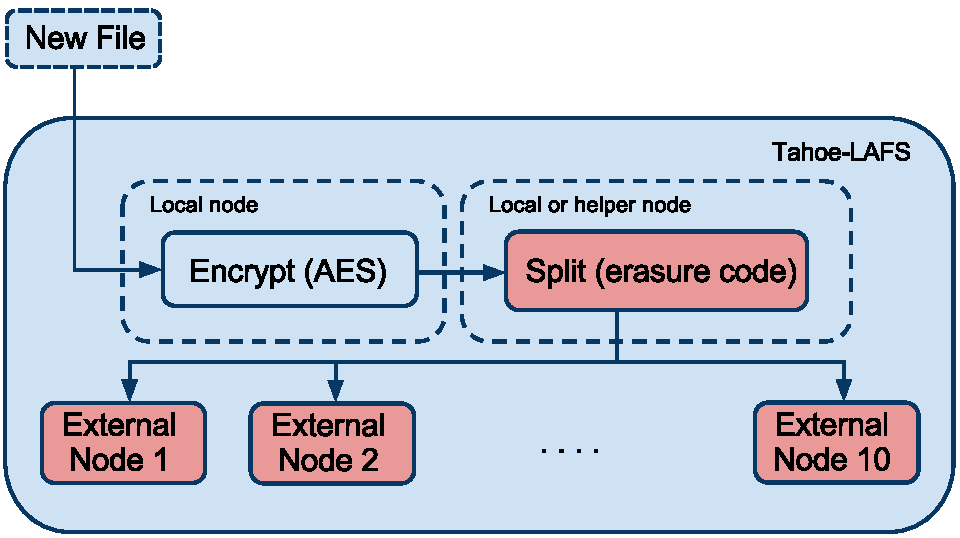
\includegraphics[width=0.9\columnwidth]{Tahoe-newfile.pdf}
    \caption{Tahoe-LAFS: Insertion of new file}
    \label{fig:tahoeinsertion}
\end{figure}

Tahoe was originally developed with funding from the former commercial web
backup service provider Allmydata, but is now a stand-alone Open
Source\footnote{GNU General Public License (GPL) version 2} project
\cite{t_ars}.  It is written in the Python programming language with the Twisted
framework, and can run on Windows, Mac OSX, Linux, Solaris and more.

\subsection{Architecture}

Tahoe has a three layer architecture: the key-value store, the filesystem, and
the application \cite{t_tahoe}.

The \textbf{key-value store}, or the ``capability-data bytes'' store, is the
lowest layer and is implemented by a grid of Tahoe-LAFS storage servers. Data is
kept on the storage servers in the form of ``shares'', which are encrypted and
encoded parts of files. Capabilities are short ASCII strings, containing
information on where to \emph{find} a file, and how to \emph{verify} it.
Nodes in the grid learn about each other through an ``introducer'', which
roughly relates to a tracker in the BitTorrent\footnote{See
\url{http://www.bittorrent.org/beps/bep\_0003.html}} protocol.

The \textbf{filesystem} layer is responsible for mapping human-meaningful
pathnames to pieces of data. Each directory contains a table of capabilities
for its children, i.e. subdirectories or files. Two forms of capabilities is
available for each file, read-only and read-write, and these can be shared to
provide shared/published directory structures with friends.

Since it is not practical for users to remember strings containing random
characters, the \textbf{application} layer is used for providing a user-friendly
interface to the directories and files.

\paragraph{File types.}

There are two kinds of files in the Tahoe-\ac{LAFS} -- \textbf{immutable} and
\textbf{mutable} files. An immutable file is created exactly once, i.e. it
cannot be modified, and can be read repeatedly. Mutable files can be modified,
and everyone who has access to the signing key can make new versions of
the mutable file.

\paragraph{Erasure coding.}

When a client puts a file on the grid, it first encrypts the file, before
breaking the file into small segments. The segments are then \emph{erasure
coded}.  The use of the Solomon-Reed erasure coding scheme, enables Tahoe to
recover a file using only a predefined subset of the parts distributed to the
storage servers, i.e. the other nodes in the grid. Erasure coding is a type of
\ac{FEC} code, which extends a message with $C$ characters into a longer message
with $N$ symbols \cite{t_reed-solomon}.  The original $C$ characters can then be
recovered from a subset of the $N$ symbols.

The properties of erasure coding can be thought of as those of replication in
\acsu{RAID} systems. \citet*{t_erasure} compare erasure coding and plain
replication, and conclude that ``\emph{...  erasure codes have mean time to
failures many orders of magnitude higher than replicated systems with similar
storage and bandwidth requirements.}''

\subsection{Use of secure hashes in Tahoe-LAFS}

\begin{figure}[!h]
    \centering
    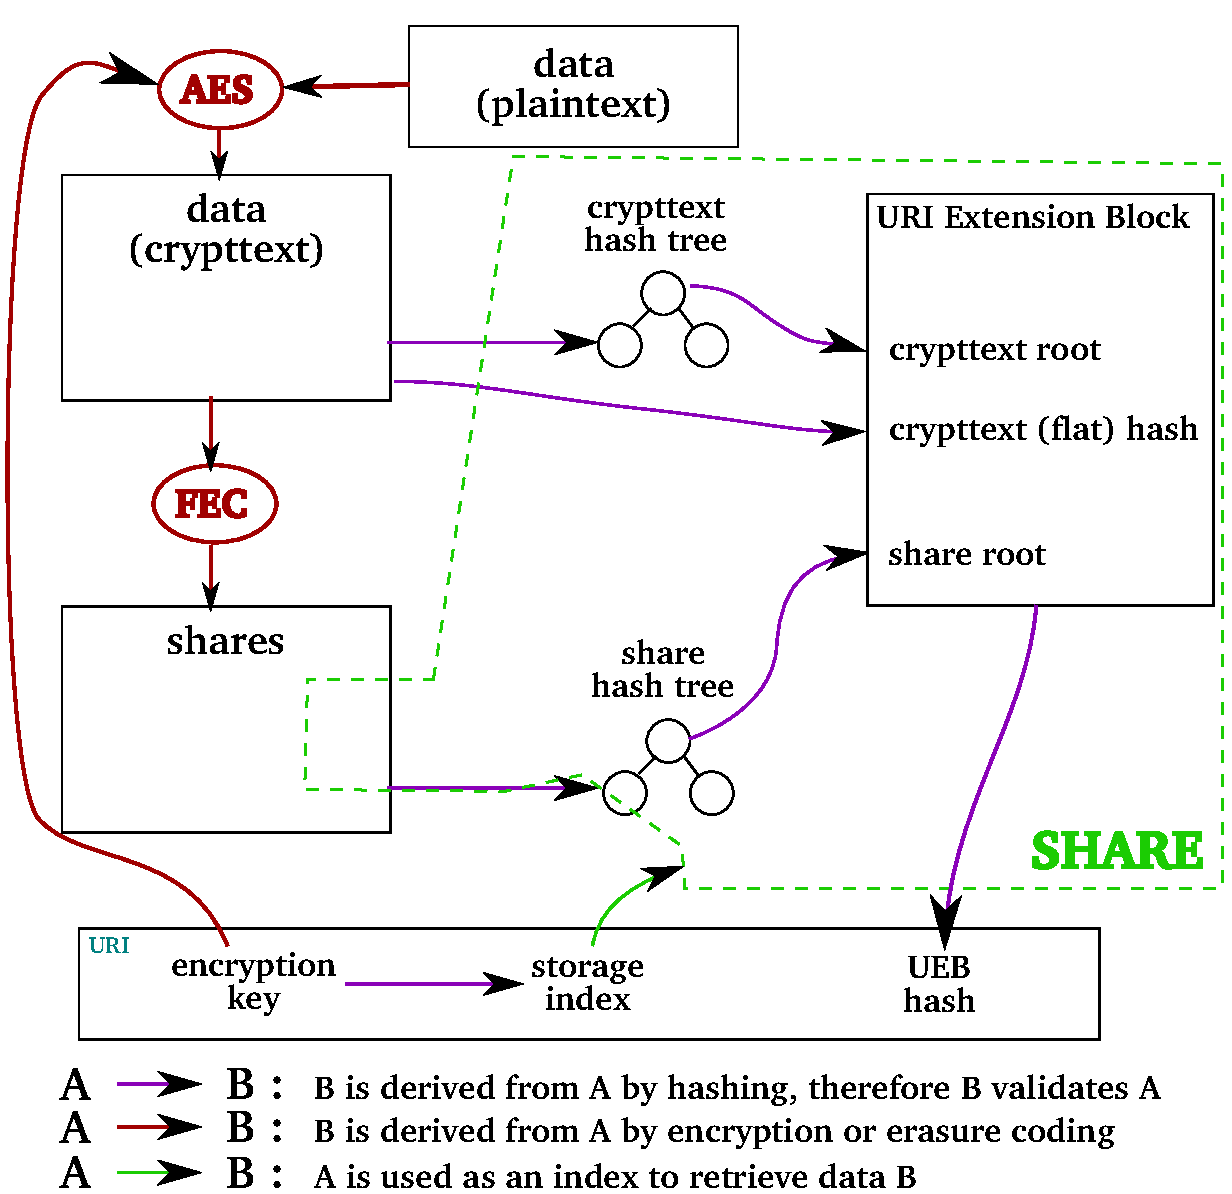
\includegraphics[width=0.9\columnwidth]{Tahoe-hashes.pdf}
    \caption{Tahoe-LAFS: Example of hashing operations.}
    \label{fig:tahoehashing}
    \emph{Figure based on
     \href{http://tahoe-lafs.org/source/tahoe/trunk/docs/specifications/CHK-hashes.svg}
     {CHK-hashes.svg from Tahoe-LAFS documentation}}
\end{figure}

As seen in Figure \ref{fig:tahoehashing}, the usage of secure hashing is
extensive in Tahoe, and has to be considered as a key part of the functionality,
and thus affecting the performance.

\paragraph{Hash Trees.}

\begin{figure}[h]
    \centering
    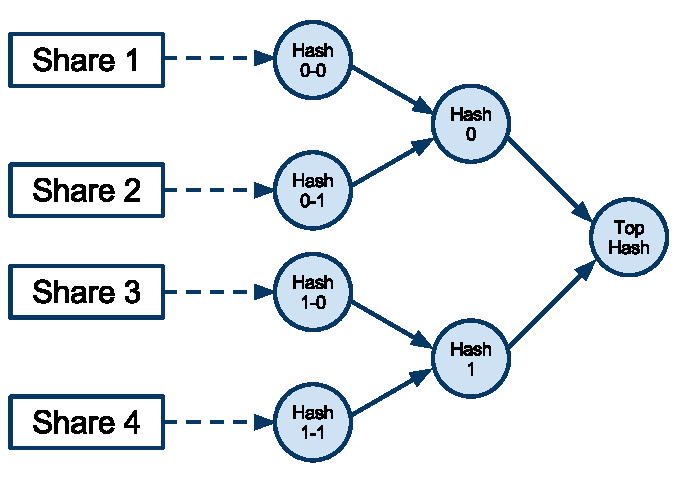
\includegraphics[width=0.9\columnwidth]{Tahoe-MerkleTree.pdf}
    \caption{Example of a Merkle tree.}
    \label{fig:tahoemerkletree}
\end{figure}

A hash tree, also known as a \emph{Merkle tree}, is a type of data structure
which can be described as a tree with nodes that can verify all information
below in the hierarchy, as depicted in Figure \ref{fig:tahoemerkletree}. This
enables Tahoe to verify small segments of a file at the time, and this can be
used for instance to start playing a movie file while it is still being
downloaded.

These secure hashes of the shares of a file, are contained within a small
data structure named the \emph{\ac{CEB}}.

\paragraph{Capabilities.}

A \textbf{capability} (or an URI) contains the encryption key, and a hash of the
\emph{\ac{UEB}}. The \ac{UEB} for each file is a data structure containing the
hash of the \ac{CEB}, the size of the file, any encoding parameters necessary to
perform the erasure decoding, and a hash of the plaintext and the encrypted
text. This is illustrated in Figure \ref{fig:tahoeueb}.

\begin{figure}[!h]
    \centering
    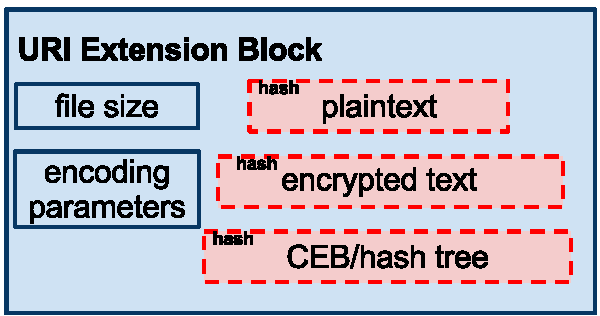
\includegraphics[width=0.9\columnwidth]{Tahoe-UEB.pdf}
    \caption{The composition of an \ac{UEB}.}
    \label{fig:tahoeueb}
\end{figure}

\paragraph{Storage Index.}

A hash of the encryption key is used to form the "storage index", which is
used for both server selection and to index shares within each storage node.
% More here?

\section{Python and Cython}

Python\footnote{\url{http://www.python.org/}} is a high-level general-purpose
programming language. Python is also an interpreted language, which means that
Python programs are compiled at runtime. There exists multiple implementations
of Python, however the most common, CPython, is implemented in C. The fact that
Python is a high-level language usually means that there are performance
penalties in contrast to lower level languages, such as C. To remedy this
problem it is possible to write extensions to the language by using the official
C-API. This approach has been used by several cryptographic libraries for
Python, such as pycryptopp\footnote{\url{http://tahoe-lafs.org/trac/pycryptopp}}
and the official hashlib\footnote{\url{http://code.krypto.org/python/hashlib/}}.

Tahoe-\ac{LAFS} is written in Python, but the SHA-3 candidate implementations found
in both the official NIST submissions and SUPERCOP are either in C or in
assembly. Therefore it is necessary to either implement the functions in Python
or make extensions to Python through the C-API, where extensions should give
the best performance.

\subsection{Cython}
Cython\footnote{\url{http://www.cython.org/}} is a language for writing Python
extensions in a language that closely resembles the Python language itself.
Basically what Cython does, is to parse Cython files and generate C source files
that utilises the Python C-API. Afterwards the generated source files can be
compiled as if they were written directly in C.

Direct calling of external C functions and methods are also supported, thus
making Cython an attractive way of wrapping external libraries written in C to
enable access from Python code.

Since the generation of C source files is an automated procedure, a small
performance trade-off is to be expected, due to the extra layer of abstraction.
The gain on the other hand, is significant in comparison to implementing
functions directly in Python.

%**************************************%
\chapter{Technical Procedure}
%**************************************%

%A bit more technical description of how we tested the candidates in Tahoe-LAFS
% - Limitations/assumptions
% - Optimized candidates.
% - Error sources.
% The points above should be taken into consideration on each section in this
% chapter.

In this chapter we will outline the procedure followed to complete our work.
Although not carried out sequentially, the problem was split up to the
following parts:

\begin{enumerate}
  \item Choose the best suiting implementations of the SHA-3 candidates.
  \item Write Python bindings, with unit tests for verification, to be able to
    use the functions from Python.
  \item Modify the Tahoe-LAFS code to utilize the SHA-3 functions.
  \item Create a method of distributing new code fast and easy to the test grid.
  \item Set up the test environment and choose test vectors.
\end{enumerate}

\section{Choosing implementations of the SHA-3 Candidates}

While the official \ac{NIST} \ac{SHA}-3 second round submissions contain both
a reference version and optimized versions of the candidates, it does not
appear to be updated since the submission deadline on September 15, 2009. They
also do not contain any benchmarking utility which could be used to decide on
the best implementation for a particular platform or architecture. \ac{SUPERCOP}
on the other hand, provides both, in combination with results stating which
compiler arguments that gives the best performance. On the downside, the
\ac{SUPERCOP} \ac{API} only specifies the {\verb crypto_hash() } function and
not an {\verb update() } function which Tahoe-\ac{LAFS} is dependent on using.

Since Tahoe-\ac{LAFS} is using \ac{SHA}-256 internally, we only test \ac{SHA}-3
functions with 256-bit output in our implementation.

\subsection{Criteria for implementation selection}

We chose the fastest implementation of each candidate that conforms to the
following criteria:
\paragraph{Criterion 1} The implementation must have an \ac{API} defined in C.
\paragraph{Criterion 2} The implementation must include a working {\verb update() } function.
\paragraph{Criterion 3} The implementation must not use assembly that can not be made
    position independent by \ac{GCC}.%FIXME: State the reason for this somewhere?
\paragraph{Criterion 4} The implementation should conform to the \acp{KAT} specified in the
    \ac{NIST} submission package, or later updates by the author.

\vspace{12pt}
Based on these criteria, we choose the fastest possible implementation based on
our benchmark in \ac{SUPERCOP} \cite{s_tahoe_supercop}. The relative speed of
each implementation, in relation to other implementation for the same and other
candidates are available at source.

\subsection{Chosen implementations}

\begin{table}
  \centering
  \begin{tabular}{ | l | l | l | }
    \hline
    \textbf{candidate} & \textbf{from} & \textbf{implementation} \\ \hline
     blake      & supercop-20101014 & blake32/ssse3 \\ \hline
     bmw        & supercop-20101014 & bmw256/optc01 \\ \hline
     cubehash   & sphlib 2.1        & c/cubehash.c  \\ \hline
     echo       & supercop-20101014 & echo256/sphlib\\ \hline
     fugue      & supercop-20101014 & fugue256/sphlib\\ \hline
     groestl    & supercop-20101014 & groestl256/sphlib\\ \hline
     hamsi      & supercop-20101014 & hamsi/simd-1  \\ \hline
     jh         & supercop-20101014 & jh256/sphlib  \\ \hline
     keccak     & supercop-20101014 & keccakc512/sseu2 \\ \hline
     luffa      & supercop-20101014 & luffa256/sse2 \\ \hline
     shabal     & supercop-20101014 & shabal256/sphlib\\ \hline
     shavite3   & supercop-20101014 & shavite3256/no-salt       \\ \hline
     simd       & supercop-20101014 & simd256/vect128 \\ \hline
     skein      & supercop-20101014 & skein256/opt           \\ \hline
  \end{tabular}
  \caption{Choosen \ac{SHA}-3 candidate implementations}
  \label{tbl:sha3:implementations}
\end{table}


The chosen implementations are shown in Table \ref{tbl:sha3:implementations}.
Their compiler flags used, which are extracted from the \ac{SUPERCOP} results,
can be seen in Table \ref{tbl:sha3:compilerflags}. Compiler flags are described
in the GCC manual\footnote{GCC Manual \url{http://gcc.gnu.org/onlinedocs/}}.
Compiler flags used for every implementation which might affect performance are:

\begin{itemize}
    \item -fomit-frame-pointer
    \item -mssse3
    \item -pthread
    \item -fPIC
\end{itemize}

It should be noted that \emph{32} in blake32 means the function works on 32-bit
words, and output a 32-byte digest (256 bit). Similarly, \emph{512} in keccakc512 
does not mean 512-bit output, but 512 bits in the internal capacity.

The relative speeds of the implementations chosen compared to
the best version in \ac{SUPERCOP}, and relative speed of the benchmark compared
to other candidates, can bee seen in Table \ref{tbl:sha3:speedrelative}.
Worth mentioning is that the fastest SHA-256 implementation in \ac{SUPERCOP} is
cryptopp\footnote{\url{http://www.cryptopp.com/}}, which is the one used by
Tahoe-\ac{LAFS}. For the most part we have found working versions of all
candidates in \ac{SUPERCOP}, however there are some exceptions.

\begin{table}
  \centering
  \begin{tabular}{ | l | l | }
    \hline
    \textbf{Candidate} & \textbf{Compiler flags}            \\ \hline
     BLAKE       & -m32 -march=native -mtune=native -O      \\ \hline
     \ac{BMW}    & -funroll-loops -m32 -march=pentium4 -O3  \\ \hline
     Cubehash    & -O2                                      \\ \hline
     Echo        & -funroll-loops -m32 -march=prescott -O2  \\ \hline
     Fugue       & -funroll-loops -O                        \\ \hline
     Grøstl      & -m32 -march=pentium3 -O                  \\ \hline
     Hamsi       & -funroll-loops -m32 -march=pentium-m -O3 \\ \hline
     JH          & -m32 -march=core2 -O                     \\ \hline
     Keccak      & -march=barcelona -O3                     \\ \hline
     Luffa       & -funroll-loops -march=k8 -O3             \\ \hline
     Shabal      & -funroll-loops -m32 -march=pentium2      \\ \hline
     Shavite3    & -funroll-loops -march=i486 -O            \\ \hline
     Simd        & -m32 -march=barcelona -O2                \\ \hline
     Skein       & -march=pentium2 -O2                      \\ \hline
  \end{tabular}
  \caption{GCC compiler flags used on the implementations}
  \label{tbl:sha3:compilerflags}
\end{table}


\begin{table}
  \centering
  \caption{Chosen SHA-3 implementations relative performance}
  \begin{tabular}{ | l | p{6cm} | r | }
    \hline
    \textbf{Candidate} & \textbf{Relative speed compared to fastest implementation} \\ \hline
     BLAKE      & 1.00                   \\ \hline
     Shabal     & 1.46                   \\ \hline
     \ac{BMW}   & 1.46                   \\ \hline
     Simd       & 1.00                   \\ \hline
     Luffa      & 1.12                   \\ \hline
     Fugue      & 2.03                   \\ \hline
     Keccak     & 1.00                   \\ \hline
     Hamsi      & 1.00                   \\ \hline
     Skein      & 2.18                   \\ \hline
     Echo       & 1.48                   \\ \hline
     Grøstl    & 3.09                   \\ \hline
     JH         & 6.19                   \\ \hline
     Shavite3   & unknown                \\ \hline
     Cubehash   & unknown                \\ \hline
  \end{tabular}
  \label{tbl:sha3:speedrelative}
\end{table}


\paragraph{JH} seems to be broken in every implementation with regard to
Criterion 2. For both the optimized versions found in \ac{SUPERCOP} and the
reference implementations in the \ac{NIST} submission package,
{\verb Hash("foofoo") } will not yield the same result as two consecutive calls
to {\verb Update("foo") }.  However the implementation in sphlib does fulfill
this requirement. We have contacted the author, Thomas Pornin, which confirms
this problem with the official JH candidate and that the author has been made
aware of the problem but has not released any updated version yet
\cite{s_pornin}.

\paragraph{Cubehash} sadly does not have a version in \ac{SUPERCOP} with a 256-bit
output, which is why we have only included a version from sphlib.

\paragraph{Simd vect128 implementation} does not by default conform to Criterion
4, because of a bug in the implementation. This has been confirmed by the author
who also supplied us with a patch to correct the bug (Gaëtan Leurent, personal
communication, November 10, 2010).

\paragraph{Blake32 \ac{SSSE3}} implementation also fail to completely fulfill
Criterion 4, however it does validate all test vectors that have a length
in bits which is a multiple of 8. Since our Python wrappers only allow (and
only need) to provide data in full bytes, we decided to keep this
implementation.

\paragraph{Shavite3} seems to have received an update\footnote{See
\url{http://www.cs.technion.ac.il/~orrd/SHAvite-3/}}. We have observed that
implementations of Shavite3 in \ac{SUPERCOP}-20101014 or later seems to fail to
verify the \ac{KAT}s, while the version we have used does. We believe this is
only because newer \ac{KAT}s will have to be generated, but since the author
has not done so, we chose to use an older version of the algorithm.

\section{Python bindings}

Since Tahoe-\ac{LAFS} is written in Python, we needed some way of interacting
with the C implementations of the NIST candidates. We did this by the use of
Cython, and built a Python object-oriented library which we named SHA3lib.
SHA3lib supports all of the 14 second round \ac{SHA}-3 candidates, but only in
their 256-bit form.

\subsection{SHA3lib}
SHA3lib is built to mimic the functionality of
hashlib\footnote{\url{http://docs.python.org/library/hashlib.html}}, the
default Python library for MD5, \ac{SHA}-1 and the \ac{SHA}-2 family. This
made us create class names for each candidate on the form
\emph{candidate name+256}. In addition, the classes included the following
functions:

\begin{itemize}
    \item Constructor with an optional data element that does the same as
    {\verb update() }
    \item {\verb update() } takes data that should be considered in hashing
    \item {\verb digest() } that produce a raw byte-digest from submitted data
    \item {\verb hexdigest() } that produce a hex representation of the digest
    \item {\verb copy() } that copies the internal state of the function and
        produces a copy of the object.
\end{itemize}

\subsubsection{Design}
Our original goal was to make SHA3lib include functionality to support all
output lengths, and not only 256-bit. This was based on our observation that
the official \ac{NIST} submission packages include ``all-in-one''
implementations that support this. Later we observed that this is not the case
for all implementations in \ac{SUPERCOP}. Together with the fact that
Tahoe-\ac{LAFS} uses 256-bit output we in the end only included support for
256-bit output in SHA3lib. The design we have used is shown in Figure
\ref{fig:python:inheritance}, and does follow the initial idea that SHA3lib
should support multiple output lengths.

\begin{figure}[h!]
    \centering
    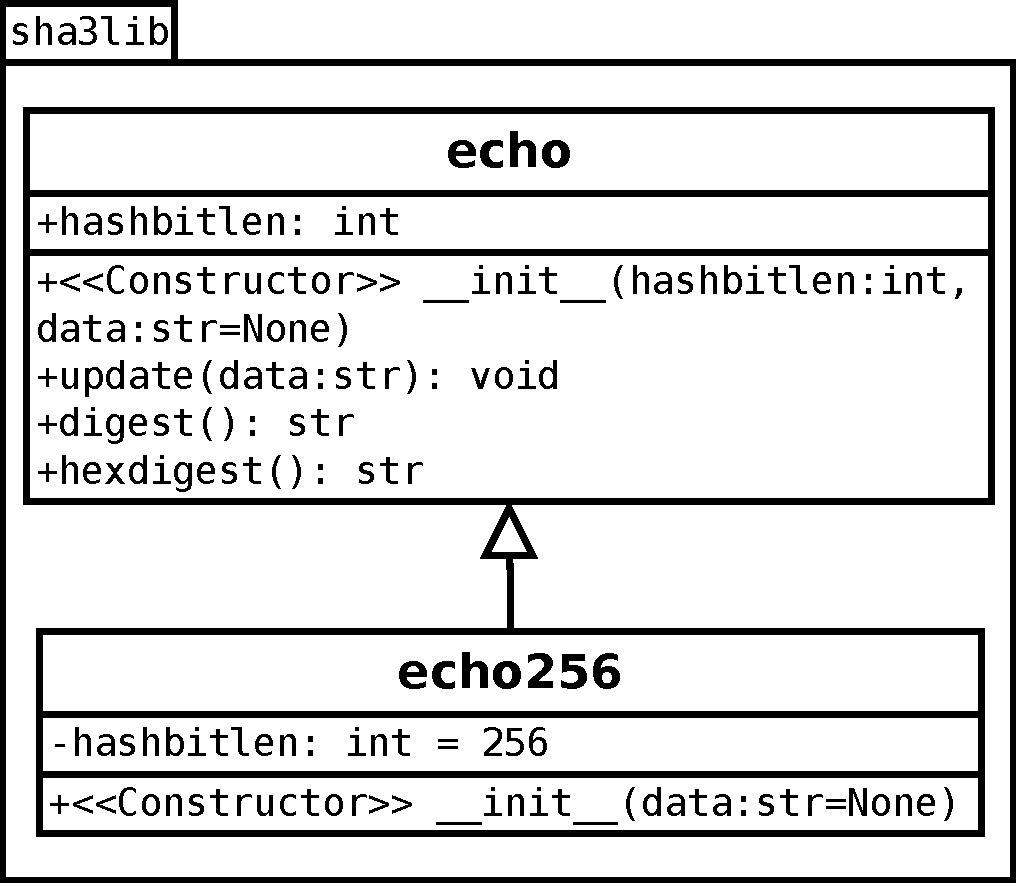
\includegraphics[width=0.6\columnwidth]{python-inheritance.pdf}
    \caption{Design of SHA3lib using echo as an example}
    \label{fig:python:inheritance}
\end{figure}

Basically the class \textbf{echo} resides in Cython and in C, and is responsible
for bringing the C functionality of the C implementation to Python. By compiling
\textbf{echo} it will be made available for use in Python.  The class
\textbf{echo256} is a simple Python class which inherits from \textbf{echo}. The
only action this class actually takes is to set the output size to 256-bit. If
the underlying C-functions would have supported multiple output sizes the same
could have been done to incorporate those.

\subsubsection{Cython}
We employ Cython to generate bindings for the C implementation and the
different candidates, as well as to create the base Python classes. To access
functions in C we need to generate a Cython header file, which pretty much does
the same as a C header file; it tells which functions and data types are
available. How we accomplish this for an implementation that satisfies the
\ac{NIST} \ac{API} is shown in Listing \ref{lst:cython_header}.

\lstinputlisting[label=lst:cython_header, caption=Cython header\, echo\_hash\_h.pxd]
{listings/echo_hash_h.pxd}

We then create a wrapper-class that mimics hashlib, this is shown in Listing
\ref{lst:cython_impl}. Functions declared with def er Python functions,
{\verb cdef } are Cython only while {\verb cpdef } are functions that can be
accessed from both. While this is just the implementation for the echo
candidate, the almost exact same pattern is used for all of the other
candidates.

\lstinputlisting[label=lst:cython_impl, caption=Cython class\, echo\_hash.pyx]
{listings/echo_hash.pyx}

\subsubsection{\ac{Distutils}}
We use \ac{Distutils}\footnote{\url{http://docs.python.org/distutils/}} to
build and install our code. The alternative to doing this would be to manually
transform Cython files to C-files, build the shared library from this and other
relevant C-files and then install by copying into the correct system directory
where Python libraries should be stored. \ac{Distutils} also support expansion
through self defined commands, something we have utilised to do Unit Testing.
Options and configuration for \ac{Distutils} is done through a file
{\verb setup.py}. Relevant configuration for compiling the echo extension, and
installing SHA3lib can bee seen in Listing \ref{lst:setup_py}.

\lstinputlisting[label=lst:setup_py, caption=Compiling echo from \ac{Distutils}]
{listings/setup.py}

\subsection{Unit tests}
We Unit Test each new candidate implementation that is included SHA3lib, both
to verify our own work and to verify that the implementation from \ac{SUPERCOP}
actually are correct. 

\paragraph{Known-Answer Tests} are used to check that the implementation conform
to the specifications of the algorithm author. The \ac{KAT}s include
bytestrings, their length and their expected message digest. The length of the
inputs range from 0 bits to 34304 bits, and also include a message that should
be repeated for about 17 million times, to verify that the implementation can handle
large inputs.

\paragraph{Basic Hash Tests} is what we have named the set of tests which test
the core basics of what a hash function implementation will have to be able to
do to be usable. This include that Init(), Update() and Final() works as
expected, and that the output is of correct size. This include that every
function should produce the same digest for the inputs Update("foofoo") and two
consecutive calls to Update("foo").

\paragraph{Copy Hash Tests} does not test any of the functionality used by
Tahoe-\ac{LAFS}, but the copy()-function is a part of Hashlib, and we have
included it in SHA3lib to conform to this. The idea is that if we have two
bytestring that share a common prefix, we can input this prefix to Update(),
then copy the state. The tests check if this is possible, and that altering the
copied state does not affect the original.


\section{Modifications to the Tahoe-\ac{LAFS} Code}
\label{sec:modtahoe}

The code of Tahoe-LAFS conforms to the style guide of Python, known as PEP 8.
This, along with the code being highly modular and consistent to its
architecture, emphasizes code readability.
With some experience using Python, it is not difficult to learn the Tahoe code
enough to understand what is happening when a file is uploaded or downloaded
with the system.

All hashing operations requested by the Tahoe system is routed through a
couple of classes and functions, and the connection to the underlying hash
function library is made on only one line. This is displayed in Listing
\ref{lst:hashutil}.

\lstinputlisting[label=lst:hashutil, caption=Extract from hashutil.py of Tahoe-LAFS source.]
{listings/hashutil.py}

As stated in Section \ref{sec:lengthextension}, none of the SHA-3 candidates is
vulnerable to the length-extension attack. Since we are interested in finding
out how Tahoe-\ac{LAFS} performs when utilizing the SHA-3 functions, we can
remove the lines that fixes the length-extension problems manually. In addition,
to try out one of the new implementations, we change line one in Listing
\ref{lst:hashutil}, and an example of this can be seen in Listing
\ref{lst:hashutilmod}.

\lstinputlisting[label=lst:hashutilmod, caption=Parts of hashutil.py of Tahoe-LAFS source after modification.]
{listings/hashutil_mod.py}

Some notes has to be made regarding the first line in Listing
\ref{lst:hashutilmod}. For every candidate we test, the whole setup and grid is
started from ground up, since changing the hash function this way cause a
backwards compatibility break, making it impossible to download files put to the
grid while using another hash function.

For the same reasons, some of the built-in unit tests of Tahoe-LAFS fail when
changing this line, because they contain test fixtures made with the included
SHA-256.  An implication of this is that uploading of mutable files renders
impossible, since the internal verification fails. For this reason, \emph{only
immutable files} are tested and measured in this paper. Implications of this are
discussed further in Chapter \ref{ch:discussion}.

\section{Automatic testing and distribution}
We fully automate the testing procedure. This is achieved by the use of
software revision control systems, which distributes both the source code of
Tahoe-LAFS, SHA3lib and shell-scripts for installation and configuration of
both. Configuration is mainly done by the use of regular expressions.

The outline of this procedure is:

\vspace{12pt}
\noindent For every \ac{SHA}-3 candidate:
        \begin{enumerate}
            \item Install SHA3lib on all nodes
            \item Replace used hash algorithm in Tahoe-LAFS with current
            candidate
            \item Install Tahoe-LAFS
            \item Create and start one Tahoe-LAFS introducer
            \item Create and start Tahoe-LAFS storage nodes on 3 nodes
            \item Create a Tahoe-LAFS client on a previously unnused node
            \item Do testing
            \item Clean up
        \end{enumerate}

\paragraph{Distribution of source code for Tahoe-LAFS and SHA3lib} is done by
\ac{SVN} and GIT respectivly. The change of hash algorithm in Tahoe-LAFS is
however done with the use of a regular expression, because of both the
simplicity of the change, and to not clutter the revision control system. Both
Tahoe-LAFS and SHA3lib uses \ac{Distutils}, which includes options to install
them globally on a system.

\section{Configuration of Test Environment}

Four machines was used as a testing grid, each containing an Intel(R) Core(TM)2
Duo E8300 \ac{CPU} and 4GB of \ac{RAM}. The 32-bit version of Ubuntu Linux
Server Edition 10.04 was the operating system of choice. The installed versions
of other relevant software can be seen in Table \ref{tbl:installedsw}.

\begin{table}[h]
  \centering
  \begin{tabular}{ | l | c | c | c | c | c | }
    \hline
    \textbf{Software} & \ac{GCC} & Cython & Python & Tahoe-\ac{LAFS} & pycryptopp \\ \hline
    \textbf{Version} & 4.4.3 & 0.13 & 2.6.5 & 1.8.0 & 0.5.25 \\ \hline
  \end{tabular}
  \caption{Installed software on the test machines.}
  \label{tbl:installedsw}
\end{table}


Tahoe-\ac{LAFS} was configured to have three storage nodes available --
\emph{shares available} -- and that only two of these had to be accessible to be
able to restore files from the grid -- \emph{shares needed}. A setting called
\emph{shares happy} was set to three storage nodes. This makes Tahoe ensure that
all storage nodes are available, so that the test environment behaves the same
for all the different tests.

The performance measurements were only performed on the Tahoe client, and not on
the storage servers. We motivated this by looking at the system performance
graphs of the storage nodes during upload and retrieval, where neither the
\ac{CPU}, network, disk or memory usage raise towards maximum threshold. The
\ac{CPU} usage during testing on one of the storage nodes is depicted in Figure
\ref{fig:munin:storagenode}.

\begin{figure}[h!]
    \centering
    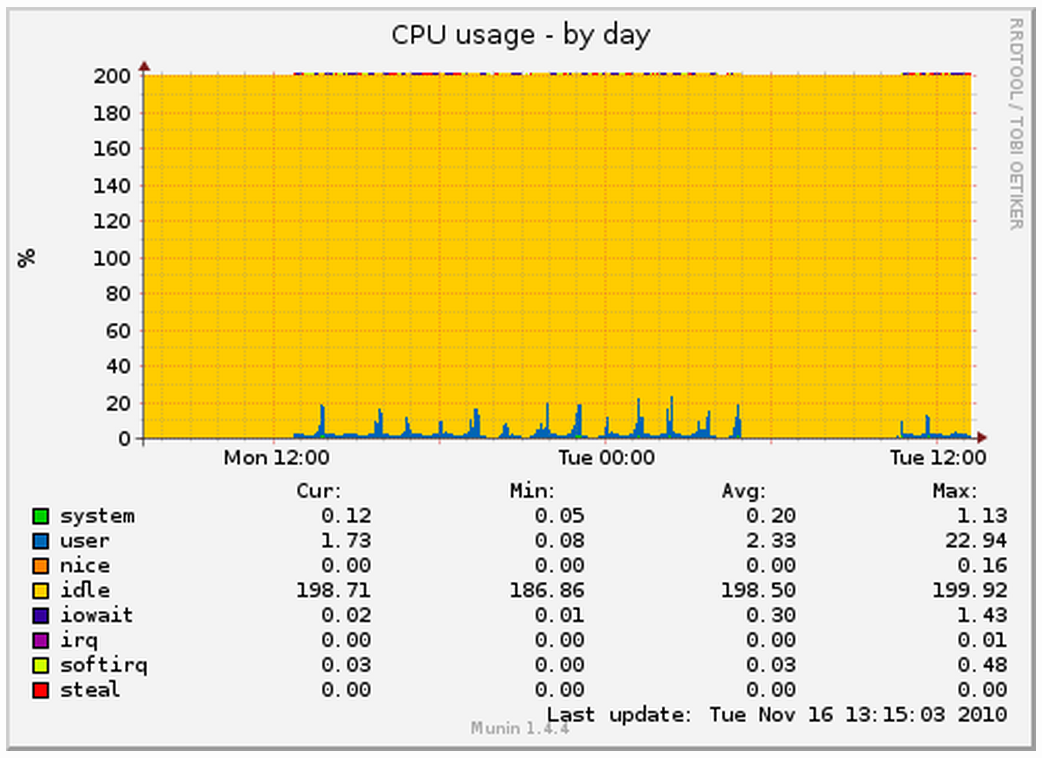
\includegraphics[width=0.8\columnwidth]{munin-tahoe05-cpuday.png}
    \caption{Graph of CPU usage during testing on a Tahoe storage node.}
    \label{fig:munin:storagenode}
\end{figure}

The tests was carried out as follows, for each of the test vectors:

\begin{itemize}
  \item Upload all files in the same category (as defined shortly) one by one.
  \item Download all files in the same manner.
\end{itemize}

During these operations, we counted the number of hashing operations performed,
and timed total time spent hashing, i.e. the total time it took for the function
calls to the underlying hashing operations to complete.

\subsection{Test Vectors}

A variety of different files was uploaded and subsequently downloaded using the
configured Tahoe grid. The numbers of the randomly generated different files
tested are shown in Table \ref{tbl:test_vectors}.

\begin{table}[h]
  \centering
  \begin{tabular}{ | l | c | }
    \hline
    \textbf{Size} & \textbf{Count} \\ \hline
    1 byte & 100 \\ \hline
    1 kilobyte & 100 \\ \hline
    1 megabyte & 50 \\ \hline
    100 megabytes & 5 \\ \hline
    1 gigabyte & 1 \\ \hline
  \end{tabular}
  \caption{Test vectors used while measuring Tahoe performance.}
  \label{tbl:test_vectors}
\end{table}


The distribution of file sizes is based on the need to test different use cases.
Although it is probably unusual to upload one byte files, this enables us to see
what happens when network delay is brought to a minimum. At the other extreme,
the one gigabyte file will show another perspective of resource utilization.

%**************************************%
\chapter{Measurements and Results}
%**************************************%

In this chapter, we will focus on the concrete results derived from our testing.
The method of testing is described, along with the test scope.

Further on, we exhibit the results from the \ac{SUPERCOP} benchmark, before
presenting the graphs of how much time the hashing operations take when
downloading and uploading a number of different test vectors, and show these
data in relation to other measurements, such as total operation time.

\section{Test scope}

As stated in Section \ref{sec:modtahoe}, only immutable files are tested. The
mutable files are not tested because of our way of integrating the SHA-3
candidates within the Tahoe-LAFS code.

To measure the performance impact of the different implementations, we time the
hash function calls from Tahoe, in addition to timing the total operation time,
e.g. the total time it takes for a 1GB file to be uploaded to grid.

\section{Measuring Performance}

Listing \ref{lst:hashutil_time} demonstrates the use of the {\verb time } module
in Python. On every call to {\verb update() } or {\verb digest() }, a variable
is increased with the time it took to run the underlying hash library
functionality. Similarly, Listing \ref{lst:testrunner} shows the use of the
{\verb date } command to calculate the number of seconds it takes it takes for
Tahoe to put a file to the grid.

\lstinputlisting[label=lst:hashutil_time, caption=Timing in Python (extraction from hashutil.py)]
{listings/hashutil_timing.py}

\lstinputlisting[language=sh, label=lst:testrunner, caption=Timing in Bash from test runner]
{listings/test_runner.sh}

\section{SUPERCOP benchmarks}
\label{sec:results:supercop}
The results of the \ac{SHA}-3 256-bit functions and \ac{SHA}-256 benchmarking in
\ac{SUPERCOP} can be seen in tables \ref{tbl:supercop:long},
\ref{tbl:supercop:4096}, \ref{tbl:supercop:1536}, \ref{tbl:supercop:576},
\ref{tbl:supercop:64} and \ref{tbl:supercop:8}. The lower the numbers, the
faster and better the algorithms performed in the test.

\begin{table}
  \centering
  \begin{tabular}{ | c | c | c | l | }
    \hline
    \textbf{Quartile} & \textbf{Median} & \textbf{Quartile} & \textbf{Function} \\ \hline
    6.01 & 6.01 & 6.02 & shabal256 \\ \hline
    6.91 & 6.94 & 7.18 & bmw256 \\ \hline
    8.37 & 8.38 & 8.43 & blake32 \\ \hline
    11.13 & 11.15 & 11.23 & simd256 \\ \hline
    13.53 & 13.53 & 13.53 & luffa256 \\ \hline
    15.45 & 15.46 & 15.50 & sha256 \\ \hline
    17.54 & 17.64 & 17.71 & fugue256 \\ \hline
    18.10 & 18.61 & 18.62 & skein256 \\ \hline
    18.95 & 18.96 & 18.98 & jh256 \\ \hline
    20.40 & 20.88 & 20.92 & keccakc512 \\ \hline
    23.36 & 23.47 & 23.48 & groestl256 \\ \hline
    29.84 & 29.96 & 30.19 & hamsi \\ \hline
    32.21 & 32.25 & 32.34 & shavite3256 \\ \hline
    32.62 & 32.64 & 32.66 & echo256 \\ \hline
  \end{tabular}
  \caption{Results from SUPERCOP: Cycles/byte for long messages}
  \label{tbl:supercop:long}
\end{table}

\begin{table}
  \centering
  \caption{Results from SUPERCOP: Cycles/byte for 4096 bytes}
  \begin{tabular}{ | c | c | c | l | }
    \hline
    \textbf{Quartile} & \textbf{Median} & \textbf{Quartile} & \textbf{Function} \\ \hline
    6.44 & 6.44 & 6.44 & shabal256 \\ \hline
    7.28 & 7.29 & 7.37 & bmw256 \\ \hline
    8.58 & 8.58 & 8.60 & blake32 \\ \hline
    11.52 & 11.52 & 11.53 & simd256 \\ \hline
    13.87 & 13.87 & 13.87 & luffa256 \\ \hline
    15.82 & 15.83 & 15.84 & sha256 \\ \hline
    18.46 & 18.63 & 18.63 & skein256 \\ \hline
    19.27 & 19.28 & 19.31 & fugue256 \\ \hline
    19.32 & 19.32 & 19.32 & jh256 \\ \hline
    21.32 & 21.49 & 21.50 & keccakc512 \\ \hline
    24.11 & 24.16 & 24.16 & groestl256 \\ \hline
    30.11 & 30.14 & 30.22 & hamsi \\ \hline
    32.76 & 32.77 & 32.77 & echo256 \\ \hline
    32.87 & 32.89 & 32.92 & shavite3256 \\ \hline
  \end{tabular}
  \label{tbl:supercop:4096}
\end{table}

\begin{table}
  \centering
  \begin{tabular}{ | c | c | c | l | }
    \hline
    \textbf{quartile} & \textbf{median} & \textbf{quartile} & \textbf{hash} \\ \hline
    7.18 & 7.18 & 7.19 & shabal256 \\ \hline
    7.59 & 7.71 & 7.82 & bmw256 \\ \hline
    8.91 & 8.92 & 8.92 & blake32 \\ \hline
    11.86 & 11.87 & 11.89 & simd256 \\ \hline
    14.43 & 14.43 & 14.64 & luffa256 \\ \hline
    16.44 & 16.45 & 16.45 & sha256 \\ \hline
    18.80 & 18.96 & 18.97 & skein256 \\ \hline
    19.89 & 19.90 & 19.91 & jh256 \\ \hline
    21.96 & 21.98 & 22.03 & fugue256 \\ \hline
    22.31 & 22.31 & 22.36 & keccakc512 \\ \hline
    25.27 & 25.28 & 25.29 & groestl256 \\ \hline
    30.36 & 30.39 & 30.60 & hamsi \\ \hline
    33.93 & 33.93 & 33.94 & shavite3256 \\ \hline
    35.90 & 35.91 & 35.95 & echo256 \\ \hline
  \end{tabular}
  \caption{Results from SUPERCOP: Cycles/byte for 1536 bytes}
  \label{tbl:supercop:1536}
\end{table}

\begin{table}
  \centering
  \caption{Results from SUPERCOP: Cycles/byte for 576 bytes}
  \begin{tabular}{ | c | c | c | l | }
    \hline
    \textbf{Quartile} & \textbf{Median} & \textbf{Quartile} & \textbf{Function} \\ \hline
    8.82 & 8.88 & 9.02 & bmw256 \\ \hline
    9.12 & 9.16 & 9.21 & shabal256 \\ \hline
    9.80 & 9.81 & 9.86 & blake32 \\ \hline
    12.91 & 12.97 & 13.00 & simd256 \\ \hline
    15.85 & 15.86 & 16.04 & luffa256 \\ \hline
    17.99 & 18.05 & 18.08 & sha256 \\ \hline
    19.95 & 19.95 & 19.97 & skein256 \\ \hline
    21.47 & 21.49 & 21.52 & jh256 \\ \hline
    25.09 & 25.12 & 25.22 & keccakc512 \\ \hline
    28.23 & 28.26 & 28.26 & groestl256 \\ \hline
    29.16 & 29.25 & 29.38 & fugue256 \\ \hline
    30.84 & 30.94 & 30.96 & hamsi \\ \hline
    36.73 & 36.76 & 36.79 & shavite3256 \\ \hline
    42.85 & 42.87 & 42.88 & echo256 \\ \hline
  \end{tabular}
  \label{tbl:supercop:576}
\end{table}

\begin{table}
  \centering
  \caption{Results from SUPERCOP: Cycles/byte for 64 bytes}
  \begin{tabular}{ | c | c | c | l | }
    \hline
    \textbf{Quartile} & \textbf{Median} & \textbf{Quartile} & \textbf{Function} \\ \hline
    21.25 & 21.25 & 21.66 & blake32 \\ \hline
    23.77 & 23.78 & 24.17 & bmw256 \\ \hline
    26.44 & 26.56 & 26.83 & simd256 \\ \hline
    32.41 & 32.53 & 32.55 & skein256 \\ \hline
    33.47 & 33.59 & 33.73 & luffa256 \\ \hline
    34.92 & 35.06 & 35.20 & shabal256 \\ \hline
    38.11 & 38.12 & 38.64 & sha256 \\ \hline
    40.11 & 40.38 & 40.38 & hamsi \\ \hline
    40.25 & 40.38 & 40.91 & jh256 \\ \hline
    50.20 & 50.34 & 50.47 & keccakc512 \\ \hline
    64.94 & 65.08 & 65.34 & groestl256 \\ \hline
    72.91 & 73.05 & 73.31 & shavite3256 \\ \hline
    101.20 & 101.33 & 101.47 & echo256 \\ \hline
    123.11 & 123.91 & 125.38 & fugue256 \\ \hline
  \end{tabular}
  \label{tbl:supercop:64}
\end{table}

\begin{table}
  \centering
  \begin{tabular}{ | c | c | c | l | }
    \hline
    \textbf{Quartile} & \textbf{Median} & \textbf{Quartile} & \textbf{Function} \\ \hline
    107.25 & 107.38 & 108.38 & blake32 \\ \hline
    114.75 & 117.88 & 119.00 & hamsi \\ \hline
    131.75 & 132.88 & 136.00 & bmw256 \\ \hline
    145.50 & 145.62 & 151.88 & luffa256 \\ \hline
    177.50 & 179.62 & 180.62 & sha256 \\ \hline
    183.88 & 184.88 & 184.88 & skein256 \\ \hline
    215.75 & 218.88 & 227.38 & simd256 \\ \hline
    226.38 & 229.50 & 232.62 & shabal256 \\ \hline
    328.25 & 329.38 & 330.38 & jh256 \\ \hline
    329.38 & 329.38 & 331.50 & shavite3256 \\ \hline
    337.88 & 339.00 & 340.00 & groestl256 \\ \hline
    399.50 & 401.62 & 404.88 & keccakc512 \\ \hline
    807.50 & 807.50 & 808.62 & echo256 \\ \hline
    855.38 & 862.75 & 874.50 & fugue256 \\ \hline
  \end{tabular}
  \caption{Results from SUPERCOP: Cycles/byte for 8 bytes}
  \label{tbl:supercop:8}
\end{table}


\subsection{Double SHA-256 Estimates}
\ac{SUPERCOP} does not measure the speed of double \ac{SHA}-256, so we have no exact
value of how many cycles this should take, we can however estimate it. For every hash
calculation double \ac{SHA}-256 will have to hash an extra 32-byte.
\ac{SUPERCOP} does not give results for hashing 32-byte, so this will also have
to be estimated. The calculations of worst-case scenario (cycles/byte for 32
byte is the same as 8 byte), best-case (cycles/byte for 32 byte is the same as
for 64 byte) and interpolation (assuming linear decrease) are shown in Table
\ref{tbl:supercop:sha256d}. The calculation for this table are as follows:

$$\frac{median * size + 179.62*32}{size} = SHA256d\ estimate (worst-case)$$

$$\frac{median * size + 38.12*32}{size} = SHA256d\ estimate (best-case)$$

$$179.62 + \frac{38.12-179.62}{64-8}*(32-8) = 118.97 (cycles/byte for 32 byte)$$

$$\frac{median * size + 118.97*32}{size} = SHA256d\ estimate (interpolation)$$

\begin{table}
  \centering
  \begin{tabular}{ | c | c | }
    \hline
    \textbf{Size} & \textbf{Median} \\ \hline
    8    & 898.1 \\ \hline
    64   & 127.93 \\ \hline
    576  & 53.85 \\ \hline
    1536 & 20.19 \\ \hline
    4096 & 17.23 \\ \hline
  \end{tabular}
  \caption{Estimates for double SHA-256}
  \label{tbl:supercop:sha256d}
\end{table}


Interpolation gives a somewhat pessimistic result of the cycles/byte needed for
hashing 32 byte, so the probable speed is somewhere in between the
interpolation point and the best case time.

\section{Measurements of Tahoe data}
\label{sec:results:tahoedata}

Tables \ref{tbl:tahoe:datauploaded} and \ref{tbl:tahoe:datadownloaded} and
describes the distribution of the different input sizes of data that
Tahoe-\ac{LAFS} sends to the hash function when uploading and downloading the
test vectors. E.g. to upload the 100 1-byte files, 15700 hashes had to be
calculated, and about 64\% of these were of size 106 byte.

For every upload Tahoe-\ac{LAFS} does, it hashes a size close to the original
file size twice. This does not happen when downloading the file.

\begin{table}
  \centering
  \caption{Distribution of data sizes hashed when uploading the test vectors.}
  \begin{tabular}{ | l | r | r | r | r | r | }
    \hline
    \textbf{Test vector}  &   1B       &  1KB      &  1MB      &  100MB    &  1GB      \\ \hline
    \textbf{Hash calls}   &   15700    &  48100    &  42200    &  49370    &  74622    \\ \hline
    \textbf{63B}          &   0\%      &  21.20\%  &  29.85\%  &  3.10\%   &  0.41\%   \\ \hline
    \textbf{101B}         &   7.00\%   &  2.91\%   &  4.97\%   &  41.58\%  &  43.92\%  \\ \hline
    \textbf{106B}         &   63.69\%  &  62.37\%  &  53.31\%  &  5.11\%   &  0.68\%   \\ \hline
    \textbf{65569B}       &   0\%      &  0\%      &  2.84\%   &  24.30\%  &  32.93\%  \\ \hline
    \textbf{131106B}      &   0\%      &  0\%      &  1.89\%   &  16.20\%  &  21.95\%  \\ \hline
    \textbf{Other}        &   29.31\%  &  13.52\%  &  0.11\%   &  7.14\%   &  9.71\%   \\ \hline
  \end{tabular}
  \label{tbl:tahoe:datauploaded}
\end{table}


\begin{table}
  \centering
  \caption{Distribution of data sizes hashed when uploading the test vectors.}
  \begin{tabular}{ | l | r | r | r | r | r | }
    \hline
    \textbf{File size} &  1B       &  1KB      &  1MB      &  100MB    &  1GB      \\  \hline
    \textbf{Total}     &  21900    &  62600    &  43400    &  28245    &  49996    \\  \hline
    \textbf{63B}       &  0\%      &  31.94\%  &  34.56\%  &  5.48\%   &  0.62\%   \\  \hline
    \textbf{101B}      &  3.65\%   &  1.59\%   &  3.57\%   &  42.76\%  &  49.16\%  \\  \hline
    \textbf{106B}      &  91.32\%  &  63.89\%  &  57.60\%  &  9.02\%   &  1.02\%   \\  \hline
    \textbf{65569B}    &  0\%      &  0\%      &  1.84\%   &  28.32\%  &  32.77\%  \\  \hline
    \textbf{131106B}   &  0\%      &  0\%      &  0.92\%   &  14.16\%  &  16.38\%  \\  \hline
    \textbf{Other}     &  5.03\%   &  2.58\%   &  1.51\%   &  0.26\%   &  0.05\%   \\  \hline
  \end{tabular}
  \label{tbl:tahoe:datadownloaded}
\end{table}


\section{Measurements of Tahoe operations}
The sum of the amount of time it took for the underlying hash library to
calculate the hash operations are exhibited in Figures \ref{fig:graph:1001b},
\ref{fig:graph:1001kb}, \ref{fig:graph:501mb}, \ref{fig:graph:5100mb} and
\ref{fig:graph:11gb}. We call this \emph{Time spent hashing}.

The numbers for uploading and downloading the different file vectors are
summarized in Tables \ref{tbl:hashingtimes:put1gb},
\ref{tbl:hashingtimes:get1gb}, \ref{tbl:hashingtimes:put100mb},
\ref{tbl:hashingtimes:get100mb}, \ref{tbl:hashingtimes:put1mb},
\ref{tbl:hashingtimes:get1mb}, \ref{tbl:hashingtimes:put1kb},
\ref{tbl:hashingtimes:get1kb}, \ref{tbl:hashingtimes:put1b} and
\ref{tbl:hashingtimes:get1b}.  The third column contains the time spent doing
other operations than hashing, i.e. \emph{Time spent not hashing = Total time -
Time spent hashing}. \emph{Fraction} displays the part of total time the calls
to the hashing libraries take.

\ac{SHA}-256 (single) is not included in the graphs, because the results were
exactly the same as for the \ac{SHA}-256d used in Tahoe-\ac{LAFS}.

As seen in Tables \ref{tbl:hashingtimes:put1gb} and
\ref{tbl:hashingtimes:get1gb}, Time spent not hashing varies between 227.37s and
252.66s during upload and 205.94s and 225.03s during download for a 1GB file.

BLAKE, \ac{BMW}, Shabal and Simd outperform \ac{SHA}-256d when both uploading
and downloading a 1GB file, but on small files, \ac{SHA}-256d is faster by a
large margin. The difference between the slowest (JH) and the fastest (BLAKE)
algorithm is 229.92s when uploading the 1GB file.

\begin{table}[h]
  \centering
  \begin{tabular}{ | l | c | c | c | c | }
    \hline
    Candidate & Total time & Time spent hashing & Difference & Fraction \\ \hline
    blake & 50.57s & 0.374s & 50.195s & .74\% \\ \hline
    bmw & 50.71s & 0.384s & 50.325s & .75\% \\ \hline
    cubehash & 50.86s & 0.727s & 50.132s & 1.43\% \\ \hline
    echo & 51.06s & 0.536s & 50.523s & 1.05\% \\ \hline
    fugue & 50.91s & 0.521s & 50.388s & 1.02\% \\ \hline
    groestl & 50.88s & 0.634s & 50.245s & 1.24\% \\ \hline
    hamsi & 51.05s & 0.436s & 50.613s & .85\% \\ \hline
    jh & 51.15s & 0.734s & 50.415s & 1.43\% \\ \hline
    keccak & 50.66s & 0.407s & 50.252s & .80\% \\ \hline
    luffa & 50.78s & 0.393s & 50.386s & .77\% \\ \hline
    sha256d & 50.16s & 0.169s & 49.990s & .33\% \\ \hline
    shabal & 50.98s & 0.402s & 50.577s & .78\% \\ \hline
    shavite3 & 50.82s & 0.456s & 50.363s & .89\% \\ \hline
    simd & 50.85s & 0.397s & 50.452s & .78\% \\ \hline
    skein & 50.99s & 0.558s & 50.431s & 1.09\% \\ \hline
  \end{tabular}
  \caption{Timing Tahoe operations: Upload of 100 1B files.}
  \label{tbl:hashingtimes:put1b}
\end{table}

\begin{table}[h]
  \centering
  \begin{tabular}{ | l | c | c | c | c | }
    \hline
    Candidate & Total time & Time spent hashing & Difference & Fraction \\ \hline
    blake & 50.32s & 0.519s & 49.800s & 1.03\% \\ \hline
    bmw & 50.33s & 0.536s & 49.793s & 1.06\% \\ \hline
    cubehash & 50.70s & 0.995s & 49.704s & 1.96\% \\ \hline
    echo & 50.57s & 0.725s & 49.844s & 1.43\% \\ \hline
    fugue & 50.56s & 0.719s & 49.840s & 1.42\% \\ \hline
    groestl & 50.62s & 0.849s & 49.770s & 1.67\% \\ \hline
    hamsi & 50.31s & 0.597s & 49.712s & 1.18\% \\ \hline
    jh & 50.72s & 0.981s & 49.738s & 1.93\% \\ \hline
    keccak & 50.35s & 0.563s & 49.786s & 1.11\% \\ \hline
    luffa & 50.34s & 0.549s & 49.790s & 1.09\% \\ \hline
    sha256d & 49.63s & 0.231s & 49.398s & .46\% \\ \hline
    shabal & 50.35s & 0.561s & 49.788s & 1.11\% \\ \hline
    shavite3 & 50.47s & 0.631s & 49.838s & 1.25\% \\ \hline
    simd & 50.34s & 0.550s & 49.789s & 1.09\% \\ \hline
    skein & 50.60s & 0.764s & 49.835s & 1.51\% \\ \hline
  \end{tabular}
  \caption{Timing Tahoe operations: Download of 100 1B files.}
  \label{tbl:hashingtimes:get1b}
\end{table}

\begin{table}[h]
  \centering
  \caption{Timing Tahoe operations: Upload of 100 1KB files.}
  \begin{tabular}{ | l | c | c | c | c | }
    \hline
    Candidate & Total time & Time spent hashing & Difference & Fraction \\ \hline
    BLAKE     &  82.90s  &  1.133s  &  81.766s  &  1.36\%  \\  \hline
    BMW       &  83.06s  &  1.164s  &  81.895s  &  1.40\%  \\  \hline
    Cubehash  &  83.96s  &  2.253s  &  81.706s  &  2.68\%  \\  \hline
    Echo      &  83.49s  &  1.669s  &  81.820s  &  1.99\%  \\  \hline
    Fugue     &  83.57s  &  1.604s  &  81.965s  &  1.91\%  \\  \hline
    Grøstl    &  83.75s  &  1.997s  &  81.752s  &  2.38\%  \\  \hline
    Hamsi     &  82.99s  &  1.326s  &  81.663s  &  1.59\%  \\  \hline
    JH        &  84.10s  &  2.287s  &  81.812s  &  2.71\%  \\  \hline
    Keccak    &  83.00s  &  1.248s  &  81.751s  &  1.50\%  \\  \hline
    Luffa     &  82.91s  &  1.193s  &  81.716s  &  1.43\%  \\  \hline
    SHA256d   &  81.83s  &  0.520s  &  81.309s  &  .63\%   \\  \hline
    Shabal    &  83.04s  &  1.204s  &  81.835s  &  1.45\%  \\  \hline
    Shavite3  &  83.27s  &  1.391s  &  81.878s  &  1.67\%  \\  \hline
    Simd      &  83.11s  &  1.214s  &  81.895s  &  1.46\%  \\  \hline
    Skein     &  83.65s  &  1.688s  &  81.961s  &  2.01\%  \\  \hline
  \end{tabular}
  \label{tbl:hashingtimes:put1kb}
\end{table}

\begin{table}[h]
  \centering
  \caption{Timing Tahoe operations: Download of 100 1KB files.}
  \begin{tabular}{ | l | c | c | c | c | }
    \hline
    Candidate & Total time & Time spent hashing & Difference & Fraction \\ \hline
    BLAKE     &  87.54s  &  1.448s  &  86.091s  &  1.65\%  \\  \hline
    BMW       &  87.59s  &  1.487s  &  86.102s  &  1.69\%  \\  \hline
    Cubehash  &  89.02s  &  2.734s  &  86.285s  &  3.07\%  \\  \hline
    Echo      &  88.33s  &  2.015s  &  86.314s  &  2.28\%  \\  \hline
    Fugue     &  88.35s  &  1.970s  &  86.379s  &  2.23\%  \\  \hline
    Grøstl    &  88.87s  &  2.335s  &  86.534s  &  2.62\%  \\  \hline
    Hamsi     &  87.90s  &  1.636s  &  86.263s  &  1.86\%  \\  \hline
    JH        &  89.11s  &  2.626s  &  86.483s  &  2.94\%  \\  \hline
    Keccak    &  87.94s  &  1.566s  &  86.373s  &  1.78\%  \\  \hline
    Luffa     &  87.76s  &  1.507s  &  86.252s  &  1.71\%  \\  \hline
    SHA256d   &  86.41s  &  0.622s  &  85.787s  &  .72\%   \\  \hline
    Shabal    &  87.80s  &  1.541s  &  86.258s  &  1.75\%  \\  \hline
    Shavite3  &  88.02s  &  1.728s  &  86.291s  &  1.96\%  \\  \hline
    Simd      &  87.97s  &  1.537s  &  86.432s  &  1.74\%  \\  \hline
    Skein     &  88.49s  &  2.055s  &  86.434s  &  2.32\%  \\  \hline
  \end{tabular}
  \label{tbl:hashingtimes:get1kb}
\end{table}

\begin{table}[h]
  \centering
  \caption{Timing Tahoe operations: Upload of 50 1MB files.}
  \begin{tabular}{ | l | c | c | c | c | }
    \hline
    Candidate & Total time & Time spent hashing & Difference & Fraction \\ \hline
    BLAKE     &  67.47s  &  1.960s  &  65.509s  &  2.90\%   \\  \hline
    BMW       &  68.32s  &  2.454s  &  65.865s  &  3.59\%   \\  \hline
    Cubehash  &  74.95s  &  9.514s  &  65.435s  &  12.69\%  \\  \hline
    Echo      &  72.99s  &  7.727s  &  65.262s  &  10.58\%  \\  \hline
    Fugue     &  71.44s  &  6.069s  &  65.370s  &  8.49\%   \\  \hline
    Grøstl    &  77.42s  &  11.50s  &  65.916s  &  14.85\%  \\  \hline
    Hamsi     &  70.04s  &  4.850s  &  65.189s  &  6.92\%   \\  \hline
    JH        &  80.56s  &  14.29s  &  66.268s  &  17.74\%  \\  \hline
    Keccak    &  69.26s  &  3.672s  &  65.587s  &  5.30\%   \\  \hline
    Luffa     &  68.59s  &  2.889s  &  65.700s  &  4.21\%   \\  \hline
    SHA256d   &  67.71s  &  2.305s  &  65.404s  &  3.40\%   \\  \hline
    Shabal    &  67.79s  &  2.165s  &  65.624s  &  3.19\%   \\  \hline
    Shavite3  &  69.78s  &  4.522s  &  65.257s  &  6.48\%   \\  \hline
    Simd      &  68.51s  &  2.483s  &  66.026s  &  3.62\%   \\  \hline
    Skein     &  72.27s  &  6.474s  &  65.795s  &  8.95\%   \\  \hline
  \end{tabular}
  \label{tbl:hashingtimes:put1mb}
\end{table}

\begin{table}[h]
  \centering
  \caption{Timing Tahoe operations: Download of 50 1MB files.}
  \begin{tabular}{ | l | c | c | c | c | }
    \hline
    Candidate & Total time & Time spent hashing & Difference & Fraction \\ \hline
    BLAKE     &  62.03s  &  1.445s  &  60.584s  &  2.33\%   \\  \hline
    BMW       &  62.19s  &  1.660s  &  60.529s  &  2.66\%   \\  \hline
    Cubehash  &  65.21s  &  5.458s  &  59.751s  &  8.37\%   \\  \hline
    Echo      &  64.15s  &  4.367s  &  59.782s  &  6.80\%   \\  \hline
    Fugue     &  63.50s  &  3.520s  &  59.979s  &  5.54\%   \\  \hline
    Grøstl    &  65.89s  &  6.100s  &  59.789s  &  9.25\%   \\  \hline
    Hamsi     &  63.04s  &  2.779s  &  60.260s  &  4.40\%   \\  \hline
    JH        &  66.63s  &  7.330s  &  59.299s  &  11.00\%  \\  \hline
    Keccak    &  62.69s  &  2.229s  &  60.460s  &  3.55\%   \\  \hline
    Luffa     &  62.35s  &  1.877s  &  60.472s  &  3.01\%   \\  \hline
    SHA256d   &  61.73s  &  1.251s  &  60.478s  &  2.02\%   \\  \hline
    Shabal    &  62.30s  &  1.569s  &  60.730s  &  2.52\%   \\  \hline
    Shavite3  &  62.78s  &  2.702s  &  60.077s  &  4.30\%   \\  \hline
    Simd      &  62.34s  &  1.695s  &  60.644s  &  2.71\%   \\  \hline
    Skein     &  63.70s  &  3.732s  &  59.967s  &  5.86\%   \\  \hline
  \end{tabular}
  \label{tbl:hashingtimes:get1mb}
\end{table}

\begin{table}[h]
  \centering
  \begin{tabular}{ | l | c | c | c | c | }
    \hline
    Candidate & Total time & Time spent hashing & Difference & Fraction \\ \hline
    BLAKE     &  127.12s  &  10.09s  &  117.02s  &  7.93\%   \\  \hline
    BMW       &  135.54s  &  14.68s  &  120.85s  &  10.83\%  \\  \hline
    Cubehash  &  194.00s  &  74.89s  &  119.10s  &  38.60\%  \\  \hline
    Echo      &  179.75s  &  62.19s  &  117.55s  &  34.60\%  \\  \hline
    Fugue     &  165.74s  &  46.62s  &  119.11s  &  28.13\%  \\  \hline
    Grøstl    &  218.60s  &  96.67s  &  121.92s  &  44.22\%  \\  \hline
    Hamsi     &  149.24s  &  36.15s  &  113.08s  &  24.22\%  \\  \hline
    JH        &  247.17s  &  123.1s  &  124.03s  &  49.81\%  \\  \hline
    Keccak    &  142.01s  &  25.00s  &  117.00s  &  17.60\%  \\  \hline
    Luffa     &  136.93s  &  18.48s  &  118.44s  &  13.49\%  \\  \hline
    SHA256d   &  137.90s  &  18.04s  &  119.85s  &  13.08\%  \\  \hline
    Shabal    &  132.47s  &  11.70s  &  120.76s  &  8.83\%   \\  \hline
    Shavite3  &  144.87s  &  31.87s  &  112.99s  &  21.99\%  \\  \hline
    Simd      &  136.44s  &  14.76s  &  121.67s  &  10.81\%  \\  \hline
    Skein     &  169.75s  &  49.70s  &  120.04s  &  29.28\%  \\  \hline
  \end{tabular}
  \caption{Timing Tahoe operations: Upload of five 100MB files.}
  \label{tbl:hashingtimes:put100mb}
\end{table}

\begin{table}[h]
  \centering
  \begin{tabular}{ | l | c | c | c | c | }
    \hline
    Candidate & Total time & Time spent hashing & Difference & Fraction \\ \hline
    BLAKE     &  116.72s  &  5.030s  &  111.68s  &  4.31\%   \\  \hline
    BMW       &  117.94s  &  6.971s  &  110.96s  &  5.91\%   \\  \hline
    Cubehash  &  143.33s  &  36.83s  &  106.49s  &  25.69\%  \\  \hline
    Echo      &  138.53s  &  30.27s  &  108.25s  &  21.85\%  \\  \hline
    Fugue     &  130.64s  &  22.41s  &  108.22s  &  17.15\%  \\  \hline
    Grøstl    &  149.91s  &  45.91s  &  103.99s  &  30.63\%  \\  \hline
    Hamsi     &  126.23s  &  17.32s  &  108.90s  &  13.72\%  \\  \hline
    JH        &  159.90s  &  57.07s  &  102.82s  &  35.69\%  \\  \hline
    Keccak    &  122.23s  &  12.09s  &  110.13s  &  9.89\%   \\  \hline
    Luffa     &  119.47s  &  9.008s  &  110.46s  &  7.54\%   \\  \hline
    SHA256d   &  120.79s  &  8.505s  &  112.28s  &  7.04\%   \\  \hline
    Shabal    &  116.80s  &  5.726s  &  111.07s  &  4.90\%   \\  \hline
    Shavite3  &  125.18s  &  15.86s  &  109.31s  &  12.67\%  \\  \hline
    Simd      &  119.00s  &  6.968s  &  112.03s  &  5.85\%   \\  \hline
    Skein     &  131.50s  &  23.86s  &  107.63s  &  18.14\%  \\  \hline
  \end{tabular}
  \caption{Timing Tahoe operations: Download of five 100MB files.}
  \label{tbl:hashingtimes:get100mb}
\end{table}

\begin{table}[h]
  \centering
  \caption{Timing Tahoe operations: Upload of one 1GB file.}
  \begin{tabular}{ | l | c | c | c | c | }
    \hline
    Candidate & Total time & Time spent hashing & Difference & Fraction \\ \hline
    BLAKE     &  253.65s  &  20.28s  &  233.36s  &  7.99\%   \\  \hline
    BMW       &  273.82s  &  29.83s  &  243.98s  &  10.89\%  \\  \hline
    Cubehash  &  388.56s  &  151.6s  &  236.89s  &  39.03\%  \\  \hline
    Echo      &  363.75s  &  126.3s  &  237.42s  &  34.72\%  \\  \hline
    Fugue     &  336.45s  &  94.99s  &  241.45s  &  28.23\%  \\  \hline
    Grøstl    &  443.01s  &  196.7s  &  246.21s  &  44.42\%  \\  \hline
    Hamsi     &  309.01s  &  75.13s  &  233.87s  &  24.31\%  \\  \hline
    JH        &  502.96s  &  250.2s  &  252.66s  &  49.76\%  \\  \hline
    Keccak    &  284.82s  &  50.48s  &  234.33s  &  17.72\%  \\  \hline
    Luffa     &  278.29s  &  37.84s  &  240.44s  &  13.59\%  \\  \hline
    SHA256d   &  273.66s  &  36.19s  &  237.46s  &  13.22\%  \\  \hline
    Shabal    &  268.31s  &  23.85s  &  244.45s  &  8.89\%   \\  \hline
    Shavite3  &  291.17s  &  63.79s  &  227.37s  &  21.90\%  \\  \hline
    Simd      &  272.52s  &  29.82s  &  242.69s  &  10.94\%  \\  \hline
    Skein     &  342.74s  &  101.3s  &  241.43s  &  29.55\%  \\  \hline
  \end{tabular}
  \label{tbl:hashingtimes:put1gb}
\end{table}

\begin{table}[h]
  \centering
  \caption{Timing Tahoe operations: Download of one 1GB file.}
  \begin{tabular}{ | l | c | c | c | c | }
    \hline
    Candidate & Total time & Time spent hashing & Difference & Fraction \\ \hline
    BLAKE     &  235.16s  &  10.12s  &  225.03s  &  4.30\%   \\  \hline
    BMW       &  235.91s  &  14.07s  &  221.83s  &  5.96\%   \\  \hline
    Cubehash  &  285.81s  &  75.16s  &  210.64s  &  26.29\%  \\  \hline
    Echo      &  275.74s  &  61.92s  &  213.81s  &  22.45\%  \\  \hline
    Fugue     &  260.50s  &  45.53s  &  214.96s  &  17.48\%  \\  \hline
    Grøstl    &  300.42s  &  94.47s  &  205.94s  &  31.44\%  \\  \hline
    Hamsi     &  252.66s  &  34.99s  &  217.66s  &  13.85\%  \\  \hline
    JH        &  321.90s  &  116.1s  &  205.79s  &  36.06\%  \\  \hline
    Keccak    &  244.55s  &  24.57s  &  219.97s  &  10.04\%  \\  \hline
    Luffa     &  237.85s  &  18.23s  &  219.61s  &  7.66\%   \\  \hline
    SHA256d   &  239.45s  &  17.34s  &  222.10s  &  7.24\%   \\  \hline
    Shabal    &  233.26s  &  11.48s  &  221.77s  &  4.92\%   \\  \hline
    Shavite3  &  252.47s  &  32.20s  &  220.26s  &  12.75\%  \\  \hline
    Simd      &  237.10s  &  14.08s  &  223.01s  &  5.93\%   \\  \hline
    Skein     &  264.67s  &  48.74s  &  215.92s  &  18.41\%  \\  \hline
  \end{tabular}
  \label{tbl:hashingtimes:get1gb}
\end{table}


\begin{figure}[h!]
    \centering
    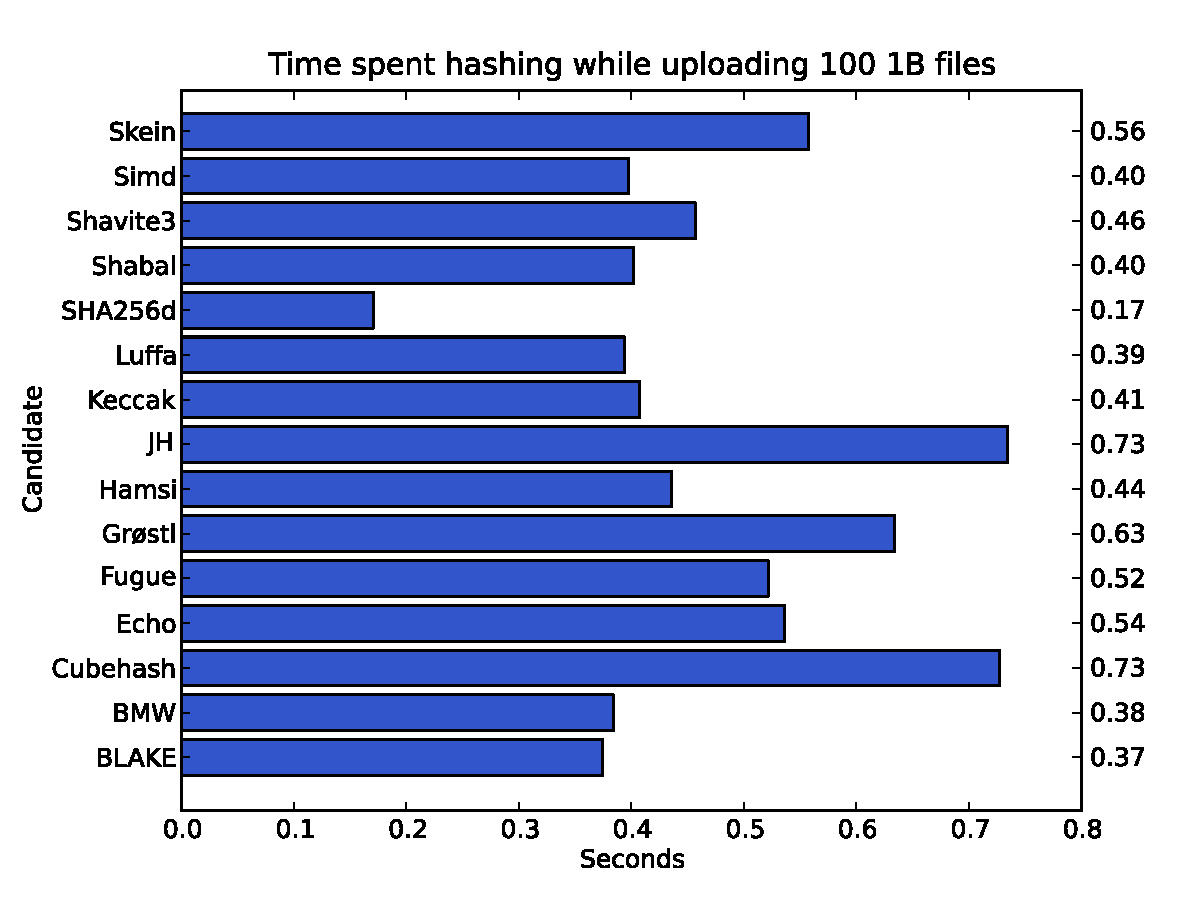
\includegraphics[width=0.9\columnwidth]
        {graphs/Timespenthashingwhileuploading1001Bfiles.pdf}
    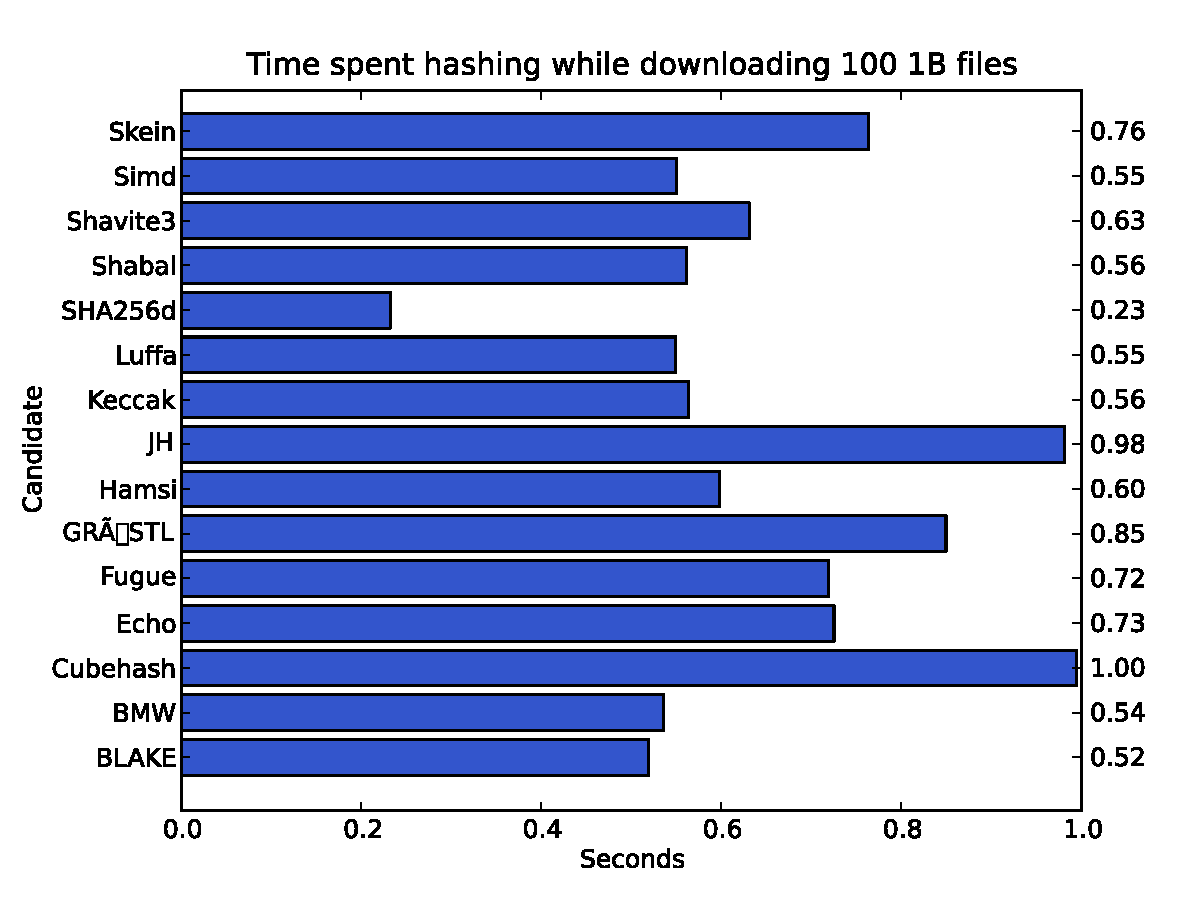
\includegraphics[width=0.9\columnwidth]
        {graphs/Timespenthashingwhiledownloading1001Bfiles.pdf}
    \caption{Figures for hash operations of 100 1B files.}
    \label{fig:graph:1001b}
\end{figure}

\begin{figure}[h!]
    \centering
    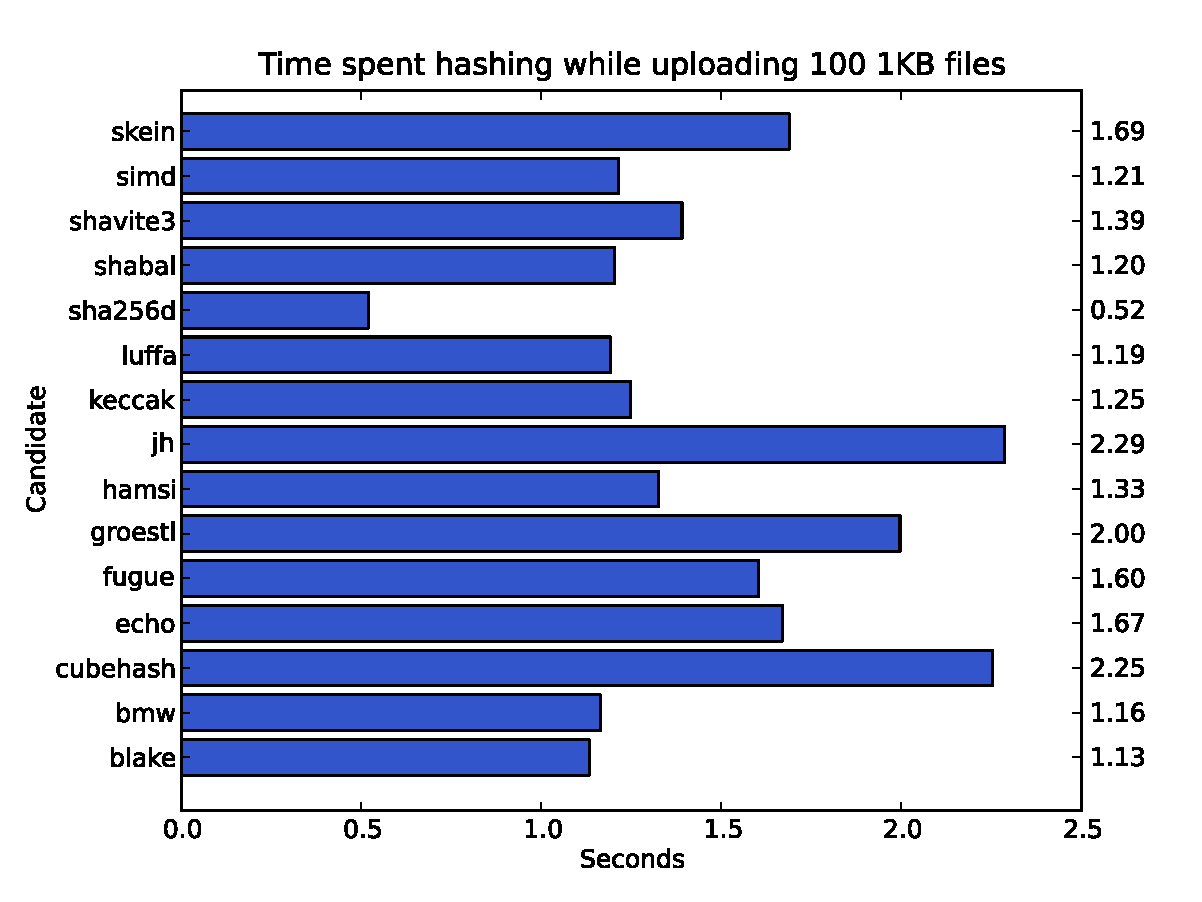
\includegraphics[width=0.9\columnwidth]
        {graphs/Timespenthashingwhileuploading1001KBfiles.pdf}
    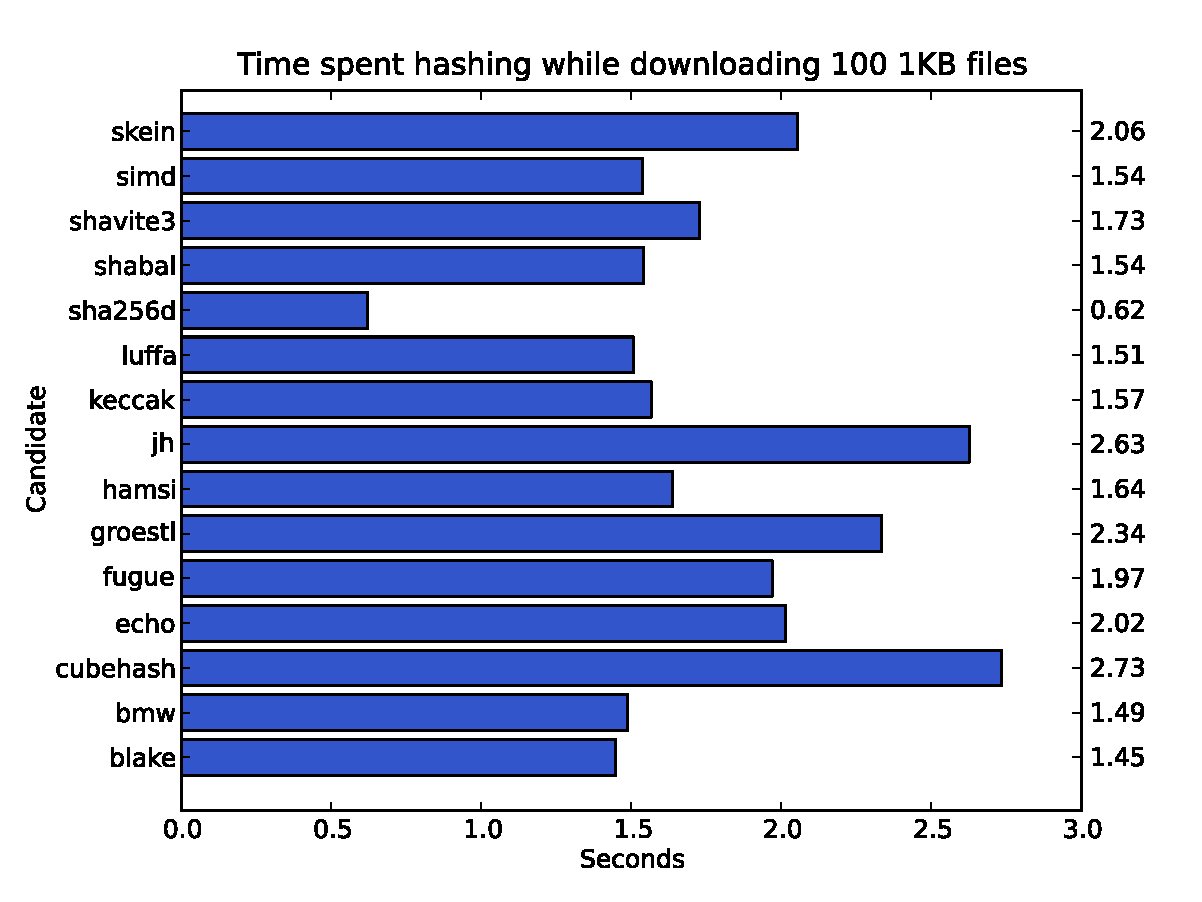
\includegraphics[width=0.9\columnwidth]
        {graphs/Timespenthashingwhiledownloading1001KBfiles.pdf}
    \caption{Figures for hash operations of 100 1KB files.}
    \label{fig:graph:1001kb}
\end{figure}

\begin{figure}[h!]
    \centering
    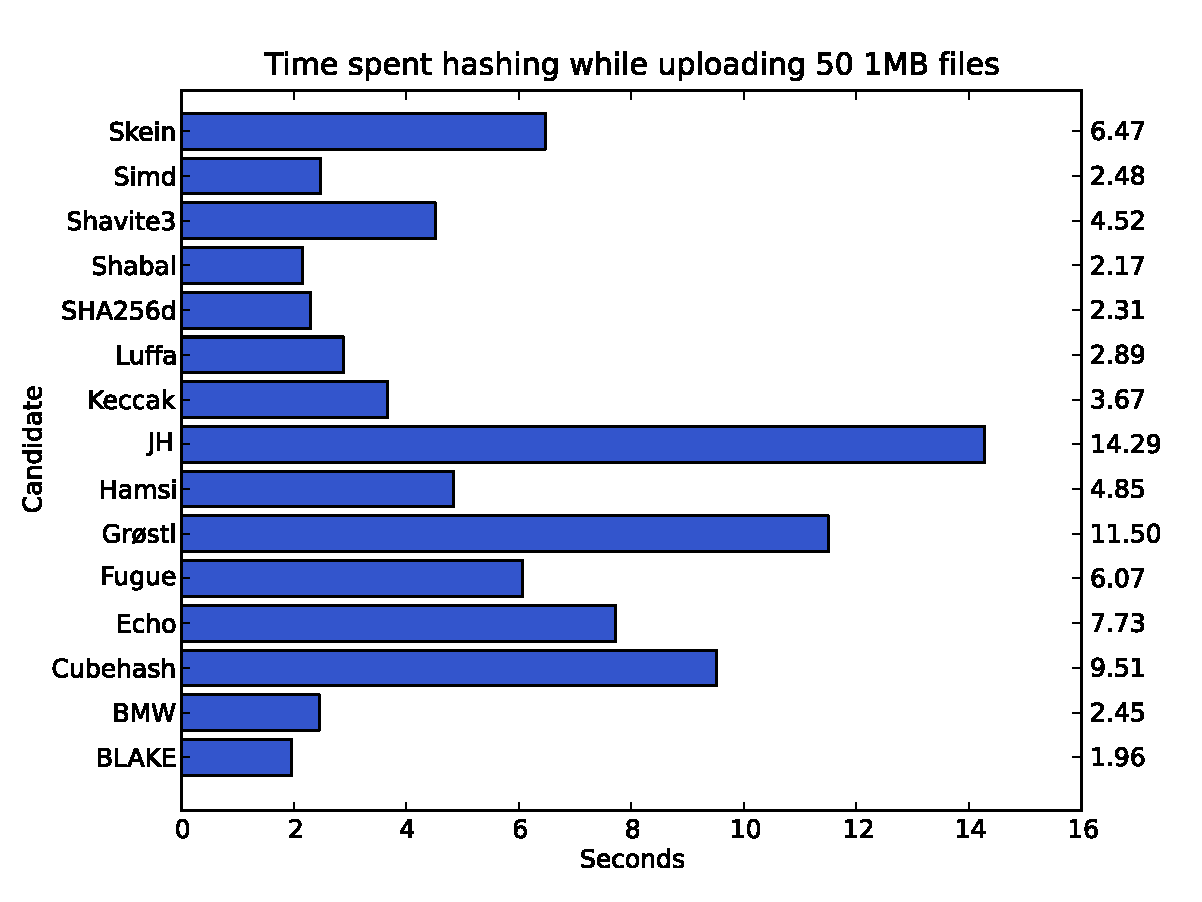
\includegraphics[width=0.9\columnwidth]
        {graphs/Timespenthashingwhileuploading501MBfiles.pdf}
    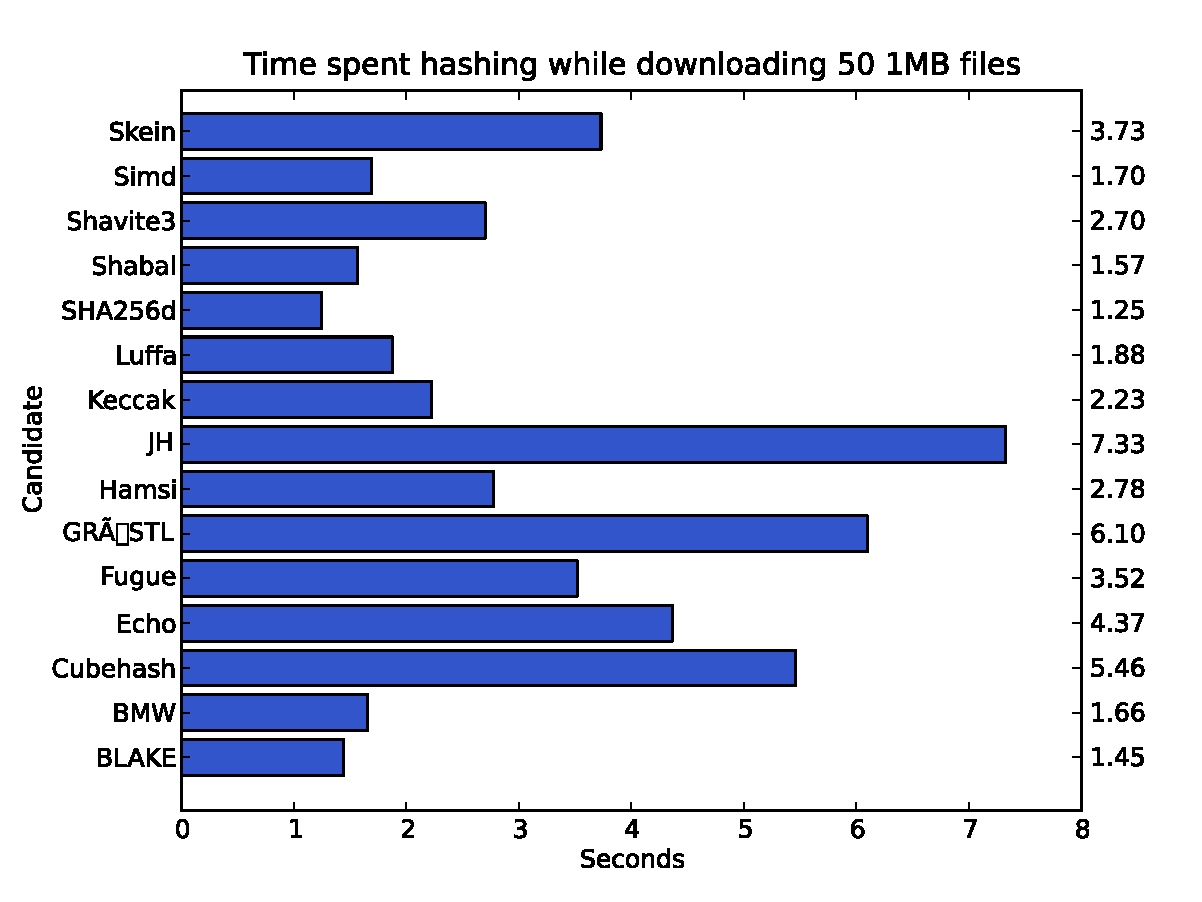
\includegraphics[width=0.9\columnwidth]
        {graphs/Timespenthashingwhiledownloading501MBfiles.pdf}
    \caption{Figures for hash operations of 50 1MB files.}
    \label{fig:graph:501mb}
\end{figure}

\begin{figure}[h!]
    \centering
    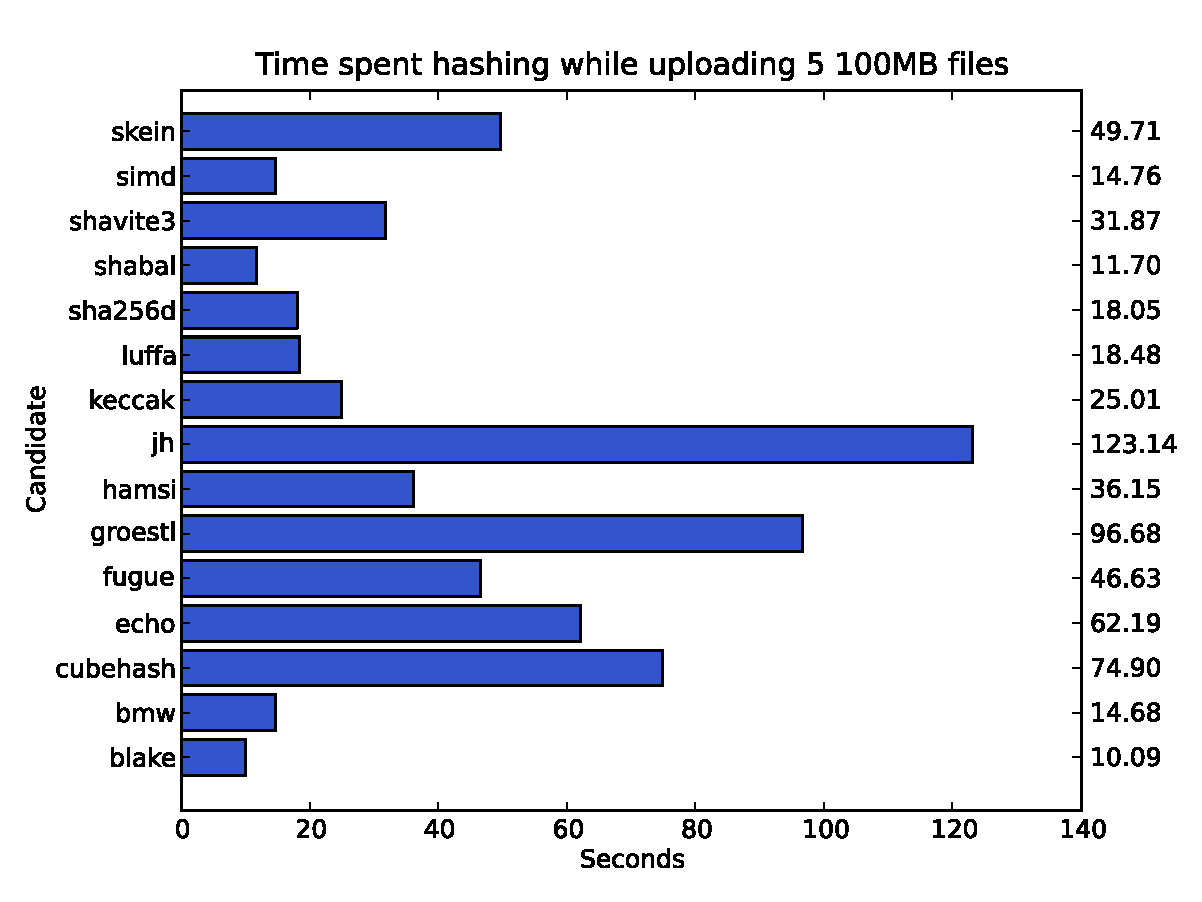
\includegraphics[width=0.9\columnwidth]
        {graphs/Timespenthashingwhileuploading5100MBfiles.pdf}
    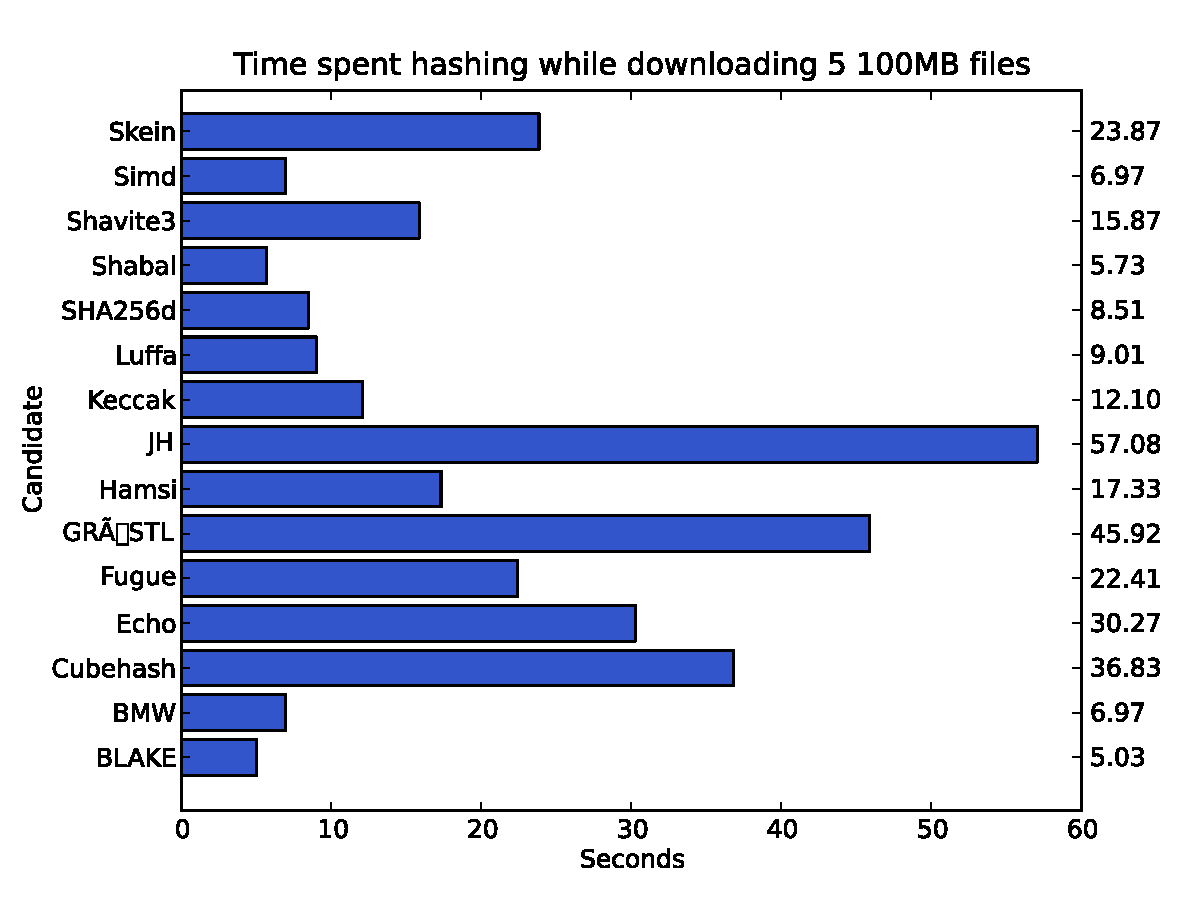
\includegraphics[width=0.9\columnwidth]
        {graphs/Timespenthashingwhiledownloading5100MBfiles.pdf}
    \caption{Figures for hash operations of five 100MB files.}
    \label{fig:graph:5100mb}
\end{figure}

\begin{figure}[h!]
    \centering
    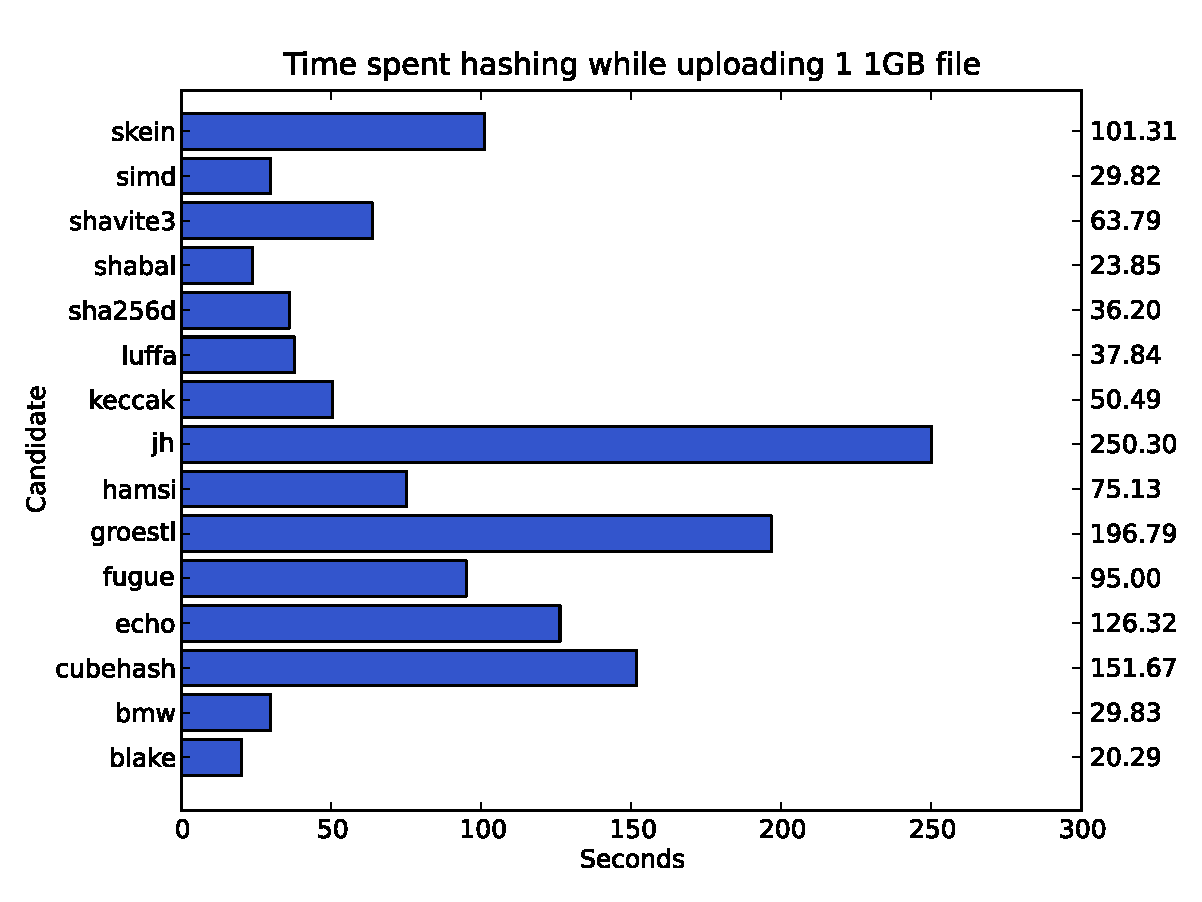
\includegraphics[width=0.9\columnwidth]
        {graphs/Timespenthashingwhileuploading11GBfile.pdf}
    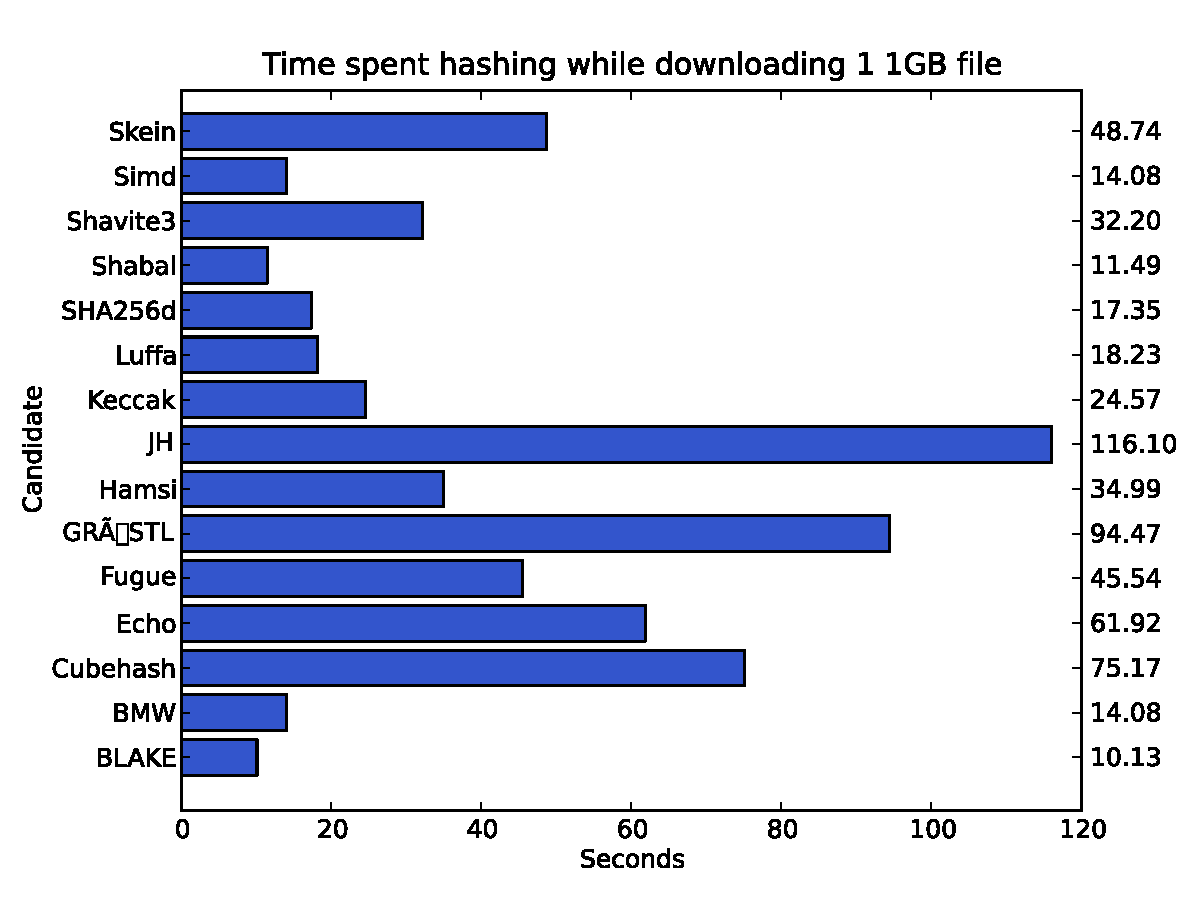
\includegraphics[width=0.9\columnwidth]
        {graphs/Timespenthashingwhiledownloading11GBfile.pdf}
    \caption{Figures for hash operations of one 1GB file.}
    \label{fig:graph:11gb}
\end{figure}

\subsection{Theoretical optimized results}
These results are calculated using the best \ac{SUPERCOP} results for each
candidate from section \ref{sec:results:supercop}, the exact sizes for each
call to the hash function from section \ref{sec:results:tahoedata}, and
interpolation to estimate the time to hash a length not recorded by
\ac{SUPERCOP}. For lengths above 4096 the results for long data lanegths are
used. The results also assume only one core of the reference processor is used.

\begin{table} 
  \centering 
  \caption{Time spent hashing during upload using best SHA-3 candidate implementations}
  \begin{tabular}{ | l | r | r | r | r | r | }
      \hline
      \textbf{Candidate} & \textbf{1B} & \textbf{1KB} & \textbf{1MB} & \textbf{100MB} & \textbf{1GB} \\ \hline
      Skein & 0.0371 & 0.1223 & 1.9918 & 18.9865 & 38.8419 \\ \hline
      Simd & 0.0256 & 0.0831 & 1.2014 & 11.3838 & 23.2786 \\ \hline
      Shavite3 & 0.0729 & 0.2368 & 3.4718 & 32.9166 & 67.3294 \\ \hline
      Shabal & 0.0247 & 0.0769 & 0.6738 & 6.1570 & 12.5713 \\ \hline
      SHA256 & 0.0363 & 0.1171 & 1.6347 & 15.4569 & 31.6126 \\ \hline
      Luffa & 0.0321 & 0.1038 & 1.4601 & 13.8123 & 28.2503 \\ \hline
      Keccak & 0.0492 & 0.1593 & 2.2527 & 21.3197 & 43.5954 \\ \hline
      JH & 0.0418 & 0.1363 & 2.0389 & 19.3538 & 39.5806 \\ \hline
      Hamsi & 0.0535 & 0.1780 & 3.1911 & 30.5509 & 62.5177 \\ \hline
      Groestl & 0.0593 & 0.1907 & 2.5415 & 23.9680 & 49.0125 \\ \hline
      Fugue & 0.0835 & 0.2581 & 2.0040 & 18.0944 & 36.9217 \\ \hline
      Echo & 0.0887 & 0.2840 & 3.5498 & 33.3515 & 68.1746 \\ \hline
      BMW & 0.0199 & 0.0633 & 0.7572 & 7.0920 & 14.4979 \\ \hline
      BLAKE & 0.0201 & 0.0650 & 0.9050 & 8.5557 & 17.4978 \\ \hline
  \end{tabular} 
  \label{tbl:tahoe:optimized_p}
\end{table}

\begin{table} 
  \centering 
  \caption{Time spent hashing during download using best SHA-3 candidate implementations}
  \begin{tabular}{ | l | r | r | r | r | r | }
      \hline
      \textbf{Candidate} & \textbf{1B} & \textbf{1KB} & \textbf{1MB} & \textbf{100MB} & \textbf{1GB} \\ \hline
      Skein & 0.0470 & 0.1216 & 0.7684 & 6.9123 & 14.1415 \\ \hline
      Simd & 0.0327 & 0.0853 & 0.4688 & 4.1447 & 8.4779 \\ \hline
      Shavite3 & 0.0938 & 0.2425 & 1.3528 & 11.9874 & 24.5205 \\ \hline
      Shabal & 0.0334 & 0.0873 & 0.2802 & 2.2453 & 4.5877 \\ \hline
      SHA256 & 0.0469 & 0.1214 & 0.6401 & 5.6296 & 11.5146 \\ \hline
      Luffa & 0.0415 & 0.1074 & 0.5713 & 5.0307 & 10.2897 \\ \hline
      Keccak & 0.0631 & 0.1645 & 0.8809 & 7.7629 & 15.8783 \\ \hline
      JH & 0.0533 & 0.1388 & 0.7929 & 7.0462 & 14.4136 \\ \hline
      Hamsi & 0.0667 & 0.1715 & 1.2209 & 11.1216 & 22.7561 \\ \hline
      Groestl & 0.0771 & 0.2000 & 1.0002 & 8.7302 & 17.8550 \\ \hline
      Fugue & 0.1137 & 0.2977 & 0.8501 & 6.6015 & 13.4832 \\ \hline
      Echo & 0.1155 & 0.3019 & 1.4069 & 12.1472 & 24.8404 \\ \hline
      BMW & 0.0262 & 0.0680 & 0.3017 & 2.5839 & 5.2835 \\ \hline
      BLAKE & 0.0261 & 0.0675 & 0.3545 & 3.1161 & 6.3735 \\ \hline
  \end{tabular} 
  \label{tbl:tahoe:optimized_g}
\end{table}


%**************************************%
\chapter{Discussion}
%**************************************%
\label{ch:discussion}

% TODO: Intro


\section{Validity of \ac{SUPERCOP} results}

Although we believe the \ac{SUPERCOP} toolkit and results give good indication
of how fast the different candidate implementations are, we do have some
comments on it.

\paragraph{Implementations does not conform to \ac{NIST} specification} for
many of the candidates. By this we mean that there is no {\verb Update() }
function available for all implementations, and that \ac{SUPERCOP} only
measures speed of hashing full byte strings. This is also a hassle for a
programmer who wants to use the implementations in \ac{SUPERCOP}

\paragraph{Incorrect implementations} are present in \ac{SUPERCOP}. By this we
mean implementations that does not conform to the \ac{KAT}s supplied.

\paragraph{Results are only valid for one specific computer}. The results we
used from \ac{SUPERCOP} are only valid for our specific computer, although it
gives an indication of which speeds can be achieved on similar computers, i.e.
32-bit. However to get a complete picture of the performance of the different
candidates one must look at different computers and architectures. This picture
might be obtained from looking at the results from all computers measured by
\ac{SUPERCOP}.

\paragraph{Extra compiler flags}
%TODO: Vi har andre compiler argumenter - dette må diskuteres
We do not compile the candidate implementation with the exact same arguments
that is used in \ac{SUPERCOP}, most notably we append the -fPIC flag. This flag
creates position-independant-code, in other words machine instruction code that
can execute properly regardless of where in memory it resides. This will make
one less register available on the x86 architecture. While we cannot directly
prove that this will affect performance of the implementations. We do however
suspect it. A person writing an optimization for \ac{SUPERCOP} will have to
balance his use of resources, among them registers, to achieve maximum speed.
The loss of one register will then give a performance penalty.  


\section{Exclusion of mutable file testing}

Since our minor change in the Tahoe-\ac{LAFS} code broke internal checks, we
were not able to test mutable files, and hence not directories.

We argue that this has minor implications for our testing results. Both because
mutable files are not applicable for most use cases, since deleting an old
version and uploading a new file gives the same functionality, and because
immutable files uses less logic and therefore are more reliable and faster in
some cases. One should bear in mind that Tahoe-\ac{LAFS} is not a revision
control system, and mutable files are not intended for this purpose.

To be able to extend the Tahoe-LAFS with new functionality to fully support new
hash functions, one have to add a new capability \cite{t_zooko}. This ensures
backwards compatibility and can be an optional feature for users to employ.
However, we found that adding a new capability was out of scope for this
assignment.

\section{Thoughts on the measurements}

\subsection{Small files}
For small files, 1B and 1KB, we can clearly see that both double \ac{SHA}-256 
greatly outperforms the \ac{SHA}-3 candidate implementations. The data being 
hashed for these files are dominated by lengths of 63 and 106 bytes. By 
comparing with \ac{SUPERCOP} results, and especially the fact that we are 
using double \ac{SHA}-256, which should result in large overhead this is
unexpected. However, we believe that the results for small files may also
reflect our use of Cython and our skill. Given large amounts of call to our
bindings, while the data processed by the actual hash functions is small and
therefore does not use a lot of time, the speed of the bindings will come in to
play.

\subsection{Large files}
For large files, 1MB, 100MB and 1GB, some of the \ac{SHA}-3 candidates are 
actually outperforming double \ac{SHA}-256, which is expected from the
\ac{SUPERCOP} results. However if we compare this result with the result for
small files, and expect that a hash algorithm should do better on a cycles/byte
basis when hashing larger data values this is not expected. Data sizes which
are hashed during 1GB and 100MB up/downloads are dominated by 101B, 65569B and
131106B. 50\% of the hashes are done on 101B, which is a size which should be
largely affected by having to do double SHA-256. However, since the small files
had a similar percentage of operations being done on 106B chunks, blaming need
to use double \ac{SHA}256 is not enough. It looks like indeed the large data
chunks being hashed is what is making the difference. If we now consider that
our bindings to the hash functions is what is causing the slow results for
small files, this makes sense. Larger amounts of data will take longer to
process for the hash function, which again results in the fraction of time used
by our bindings is decreased.


%FIXME: Nevn noe en plass om at vi kanskje burde timet kallene til HASH
%funksjonen også.
\subsection{Impact of double \ac{SHA}-256}
The impact of using double \ac{SHA}-256 compared to single is suprisingly
small, even if you use the best-case estimate from Table
\ref{tbl:supercop:sha256}. For 1B, 1KB and 1MB files the data hashed is almost
exclusively 106B or less. If we assume data is hashed at the performance of 576
bytes, single \ac{SHA}-256 should outperform double \ac{SHA}-256 by about 10\%.
For 1B files this difference is eaten up by external factors (other
processes), the same goes for 1KB files. For 1MB files, there seems to be a
difference, however this difference is so small that we deem it unimportant.
For the larger files the performance penalty is even smaller, so all in all we
deem the performance penalty for Tahoe-\ac{LAFS} for using double \ac{SHA}-256
as opposed to single unimportant.

\subsection{The candidates}
If we look primarily at the large file up/download we see that the candidates
that outperforms, or are close to outperforming \ac{SHA}-256 are BLAKE,
\ac{BMW}, Shabal, Simd and Luffa. This is expected and corresponds with the
results from \ac{SUPERCOP}.  

\subsection{Final round candidates}
BLAKE, Keccak, Skein, Grøstl and JH have made it through to the final round of
the \ac{SHA}-3 competition. %TODO: some comments on theese

\subsection{Optimizing results}
We have not used the fastest possible implementations possible for various
reasons mentioned previously. However, if we had actually used the fastest
implementations in \ac{SUPERCOP}, achieved median speed for every hash
calculated the results should look as in Table X. The table is calculated using
the lengths of data actually hashed by Tahoe-\ac{LAFS}, the medians from
\ac{SUPERCOP} results, and interpolation for sizes in between those mentioned in
\ac{SUPERCOP}. The point of this result is to see the maximum performance gain
possible for TAHOE-\ac{LAFS} by adopting one of the current \ac{SHA}-3
candidate implementations.

%TODO: Optimaliserte resultater tabell

% Describe inconsistencies in the numbers, and try to explain them.
% Time spent not hashing varies because: Variable use of CPU regs?
%
% Compare our results with general (SUPERCOP) results.
%
% How much gain can Tahoe-LAFS get by switching to SHA-3?
%
% Drag in the five selected remaining candidates.

\section{Improvement of methods}
% More general stuff. What could have been done differently? Criticize
% ourselves.
%
% Optimized candidates - which gain could be expected from more optimized
%   candidates?

\subsection{The use of Cython}

The Python-bindings generated for Cython in C are not necessarily the most
optimized versions possible to write and they are ugly to read or change (from
a C perspective). However we consider them to be good enough, and they are
equal for all the \ac{SHA}-3 candidates which means they should give the same
performance penalty. The \ac{SHA}-256 version will of course not suffer from
the same penalty, however we believe the possible performance gain is small.
This is due to the fact that no intensive operations take place in our
Cython-code.

The alternative would be creating manual Python-bindings for all the candidates
which would require a lot more work on our side, especially given the lack of a
good enough and common \ac{API} for the implementations in \ac{SUPERCOP}.
Another fact important for this decision was that we did not know exactly which
implementation of each candidate we would end up using, and we ended up trying
several for most candidates.

\subsection{Faster implementations}
We do not claim to have tested the fastest possible nor existing version
of most of the candidates. We are certain that someone of more skill and
knowledge about the inner workings of the \ac{SHA}-3 candidates, \ac{GCC} and
Python could make significantly faster implementation.

\subsection{Test with different Erasure Coding schemes}
By default Tahoe-\ac{LAFS} comes with a coding scheme of 3-7-10 (shares needed,
shares happy, shares total) while we test with a configuration of 2-3-3. It
would have been interesting to see how this (and other schemes) would affect
both the overall performance and the percentage of time spent hashing.

\subsection{Measure with real use cases}
Our test use random generated data of a certain length. In a real use case for
Tahoe-\ac{LAFS} the data would probably be both of varying length, and of
lengths not tested by us. In a real use case both a feasible erasure coding
scheme would have to be decided, and the files would represent what you
actually would want to use Tahoe-\ac{LAFS} for.

%**************************************%
\chapter{Conclusion and Future Work}
%**************************************%

% This chapter should contain:
% -----------------------------------------------------------
% A somewhat short conclusion summing up what has been done, and results and
% discussion

We had hoped to contribute more to the Open Source project Tahoe-LAFS, when
starting on our assignment. It was early evident that implementing a new
capability was out of scope, since creating Python bindings and trying out
new implementations was prioritized. Future work should implement the support
for choosing hashing algorithm in a proper manner which ensures backwards
compatibility.

Four of the candidates has been shown to perform better than the currently used
SHA-256 -- BLAKE, BlueMidnightWish, Shabal and Simd. The time it takes for
Tahoe-LAFS to upload a one gigabyte file, could improve by $5\%$ if the best
performing SHA-3 candidate, BLAKE, were to be used. One has to bear in mind that
SHA-256 has been optimized and tweaked for a number of years, and that these
performance differences undoubtedly will continue to increase as new and better
implementations will be developed for the final chosen \ac{SHA}-3 algorithm.

Perhaps the most important finding in this project, is that the SUPERCOP
benchmarking indeed drives the development of new and better implementations
forward, but since the SUPERCOP \ac{API} does not conform to the \ac{NIST}
\ac{API}, the developers leave important functionality out (i.e.
{\verb update() }), and hence make it difficult for people who wish to try out
and test the \ac{SHA}-3 candidates in real world applications.

% BibTeX bibliography lives in external file
\bibliographystyle{plainnat}
\bibliography{ref_sha3,ref_tahoe}

% Uncomment to enable appendices.
%\appendix
%\appendixpage
%\addappheadtotoc

% Use ordinary \chapters from here on..

\end{document}
